\documentclass[11p,aspectratio=169]{beamer}

\geometry{paperwidth=160mm,paperheight=120mm}

\usetheme[{titleformat plain}=smallcaps,
           titleformat title=smallcaps,
           titleformat subtitle=regular,
           titleformat section=smallcaps,
           titleformat frame=smallcaps,
        %    numbering=fraction,
          ]{metropolis}

\usepackage{style/main}
\usepackage[T1]{fontenc}
\usepackage[english]{babel}
\usepackage{graphicx}
\usepackage{tcolorbox}
\usepackage{xcolor}
\usepackage{amsmath,bm,amsfonts,amssymb,array,calc,amsthm,rotating,amscd,bbm}
\usepackage{url}
\usepackage{hyperref}
\usepackage{fontawesome}
\usepackage{movie15}
\usepackage{tikz}
\usepackage{multicol}
\usepackage{wrapfig}
\usetikzlibrary{quantikz}
% in documenet


\usefonttheme[onlymath]{serif}
\usepackage[absolute,overlay]{textpos}

\setbeamerfont{caption}{size=\scriptsize}
% \usepackage[natbib=true,backend=biber,useprefix=true]{biblatex}
% \addbibresource{references.bib}
% \setbeamercolor{bibliography item}{parent=palette primary}
% \setbeamercolor*{bibliography entry title}{parent=palette primary}

% \usetheme[progressbar=frametitle]{metropolis}
% \setbeamertemplate{frame numbering}[fraction]
% \metroset{background=dark}
% \definecolor{primary}{RGB}{245, 10, 10}
% \setbeamercolor{palette primary}{bg=white, fg=black}
% \setbeamercolor{background canvas}{parent=palette primary}
% \setbeamercolor{normal text}{fg=black}
% \setbeamercolor{progress bar}{use=palette primary, fg=primary}
% natbib=true,style=authoryear,backend=bibtex,useprefix=true
% \setbeamerfont{caption}{size=\tiny}

% \usepackage[style=authoryear]{biblatex}
%%% THIS ADDS THE COMMA BETWEEN AUTHOR NAME AND YEAR
% \renewcommand*{\nameyeardelim}{\addcomma\space}
% \addbibresource{test.bib}


\title{Towards a hybrid quantum operating system}
\subtitle{First Year PhD students workshop}
\author{Andrea Pasquale}
\date{30th September 2022}
\titlegraphic{
    \vspace*{11.5cm}
    \raisebox{20pt}[10pt][10pt]{
\includegraphics[height=4cm]{../logos/unimi_logo.pdf}}\hspace*{30pt}
    \raisebox{20pt}[10pt][10pt]{
\includegraphics[height=4cm]{../logos/tii_logo.png}}\hspace*{30pt}
    \raisebox{20pt}[10pt][10pt]{
\includegraphics[height=4cm]{../logos/infn_logo.png}}\hspace*{30pt}
    % \includegraphics[height=1.3cm]{../_logos/erc_logo1.png}

    % \vfill\vspace*{230pt}
    % 
\includegraphics[height=1cm]{../_logos/unimi_logo.png}\hfill
    % 
\includegraphics[height=1cm]{../_logos/infn_logo.png}\\
    % \vspace*{5pt}
    % {
    %     \fontsize{3pt}{3.5pt}\selectfont
    %     \begin{center}
    %         This project has received funding from the European Union's Horizon
    %         2020 research and innovation programme under grant agreement No
    %         % 740006\quad \includegraphics[height=5pt]{../_logos/eu-flag.jpg}
    %     \end{center}
    % }
}


\begin{document}

\maketitle

% \begin{frame}{Outline}
%     Using a quantum device is not easy 
% \end{frame}

\begin{frame}
    \begin{figure}
        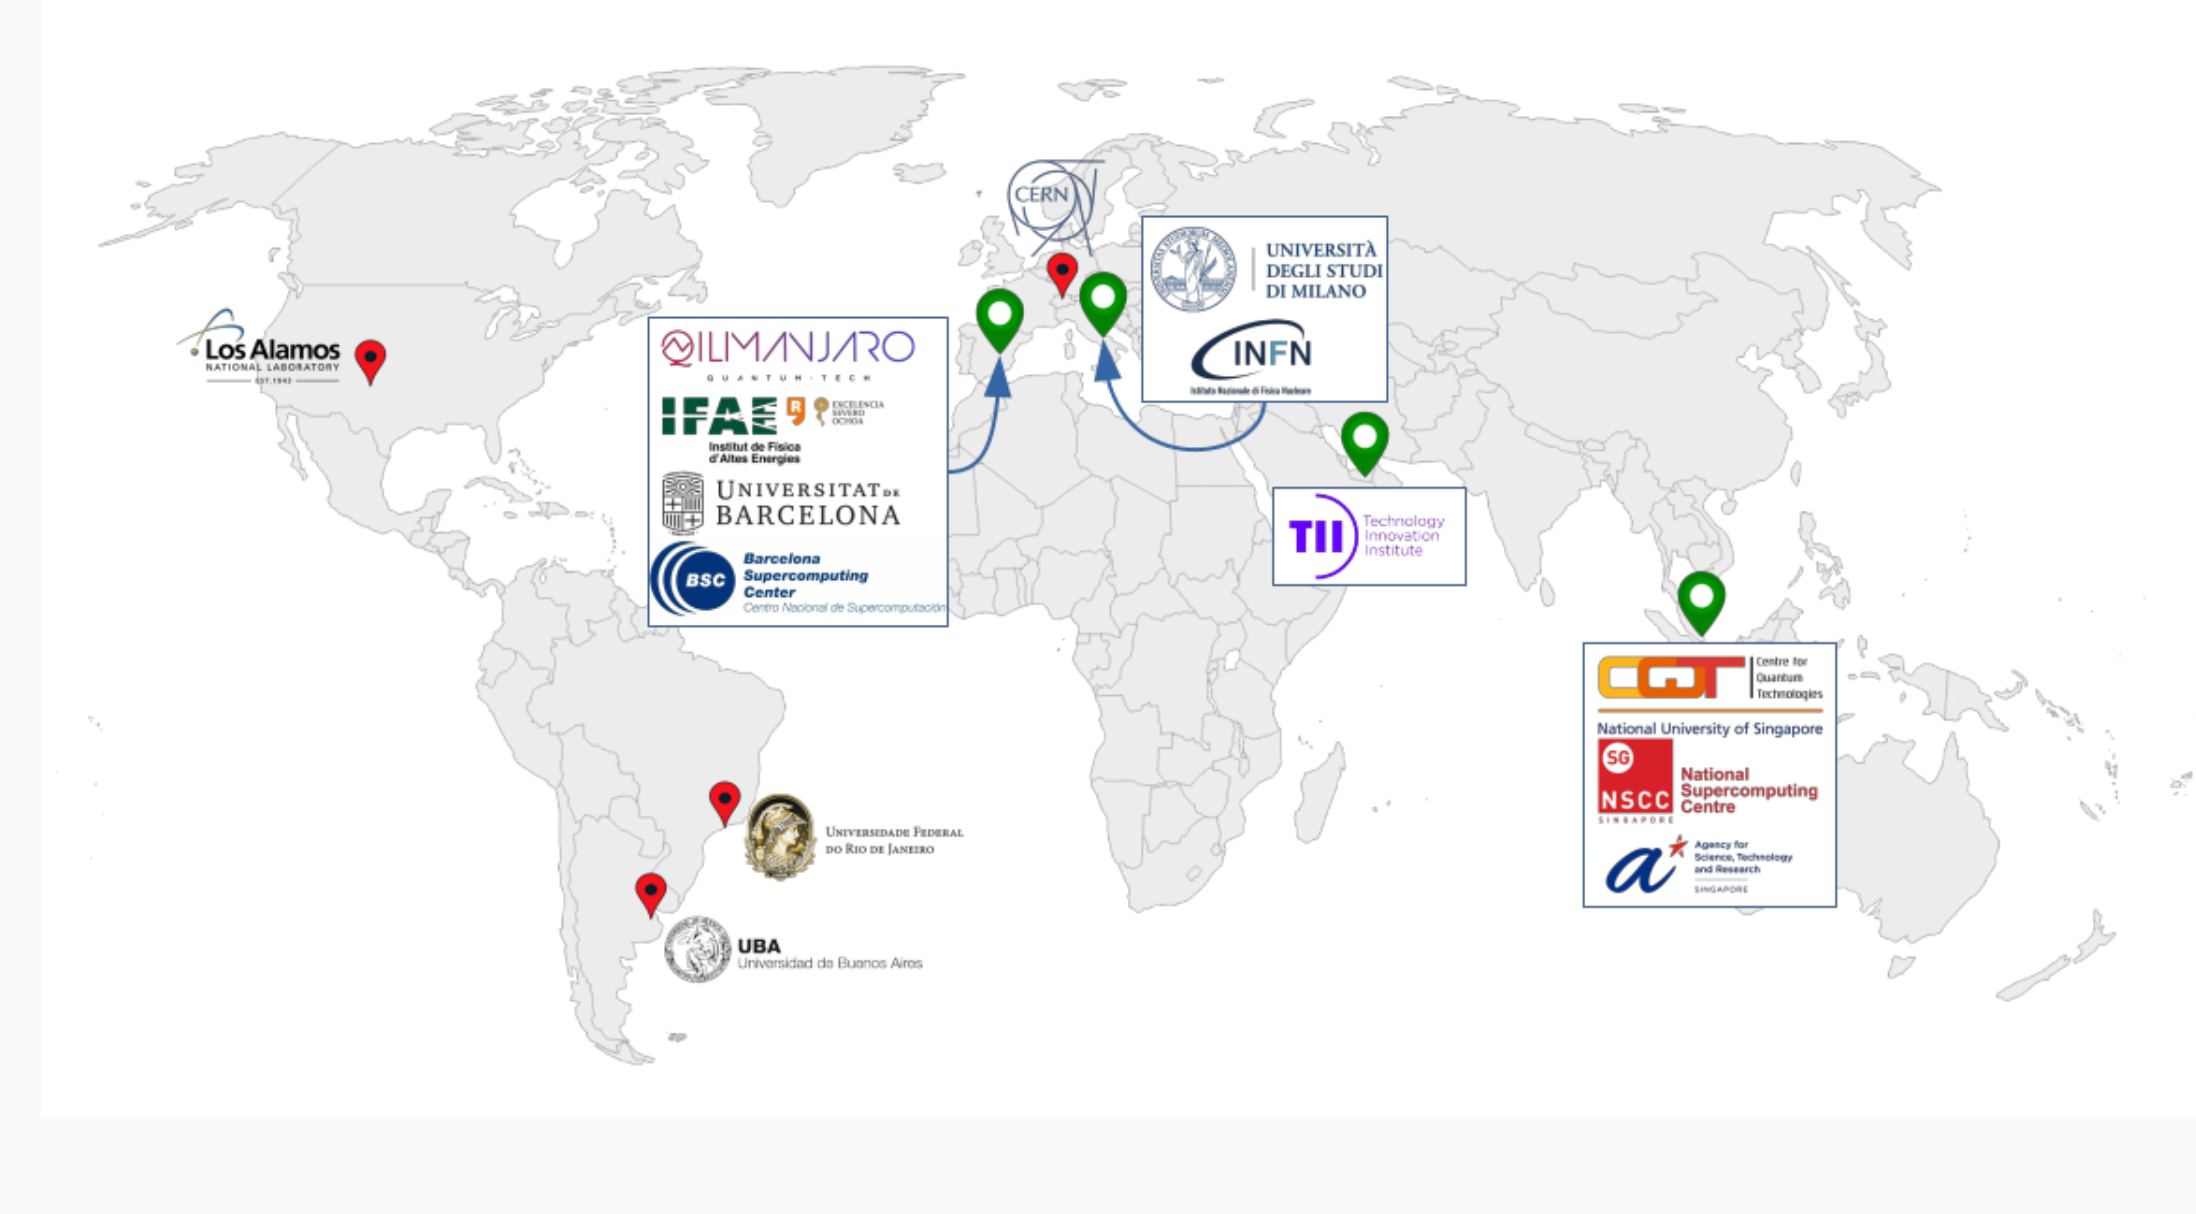
\includegraphics[width=\textwidth]{figures/map.png}
    \end{figure}
    % \begin{columns}
    %     \begin{column}[0.5 \textwidth]
        \begin{multicols}{2}
            \begin{itemize}
                \item Chips with 1 and 5 qubits at TII
                \item Chips with 1 and 2 qubits at Qilimanjaro
                \item Chip with 1 qubit in Italy (soon)
                \item Chips with up to 10 qubits at CQT
            \end{itemize}
        \end{multicols}
    %     \end{column}
    %     \begin{column}[0.5 \textwidth]
    %         test
    %     \end{column}
    % \end{columns}
\end{frame}

\begin{frame}{Challenge}
    \begin{figure}
        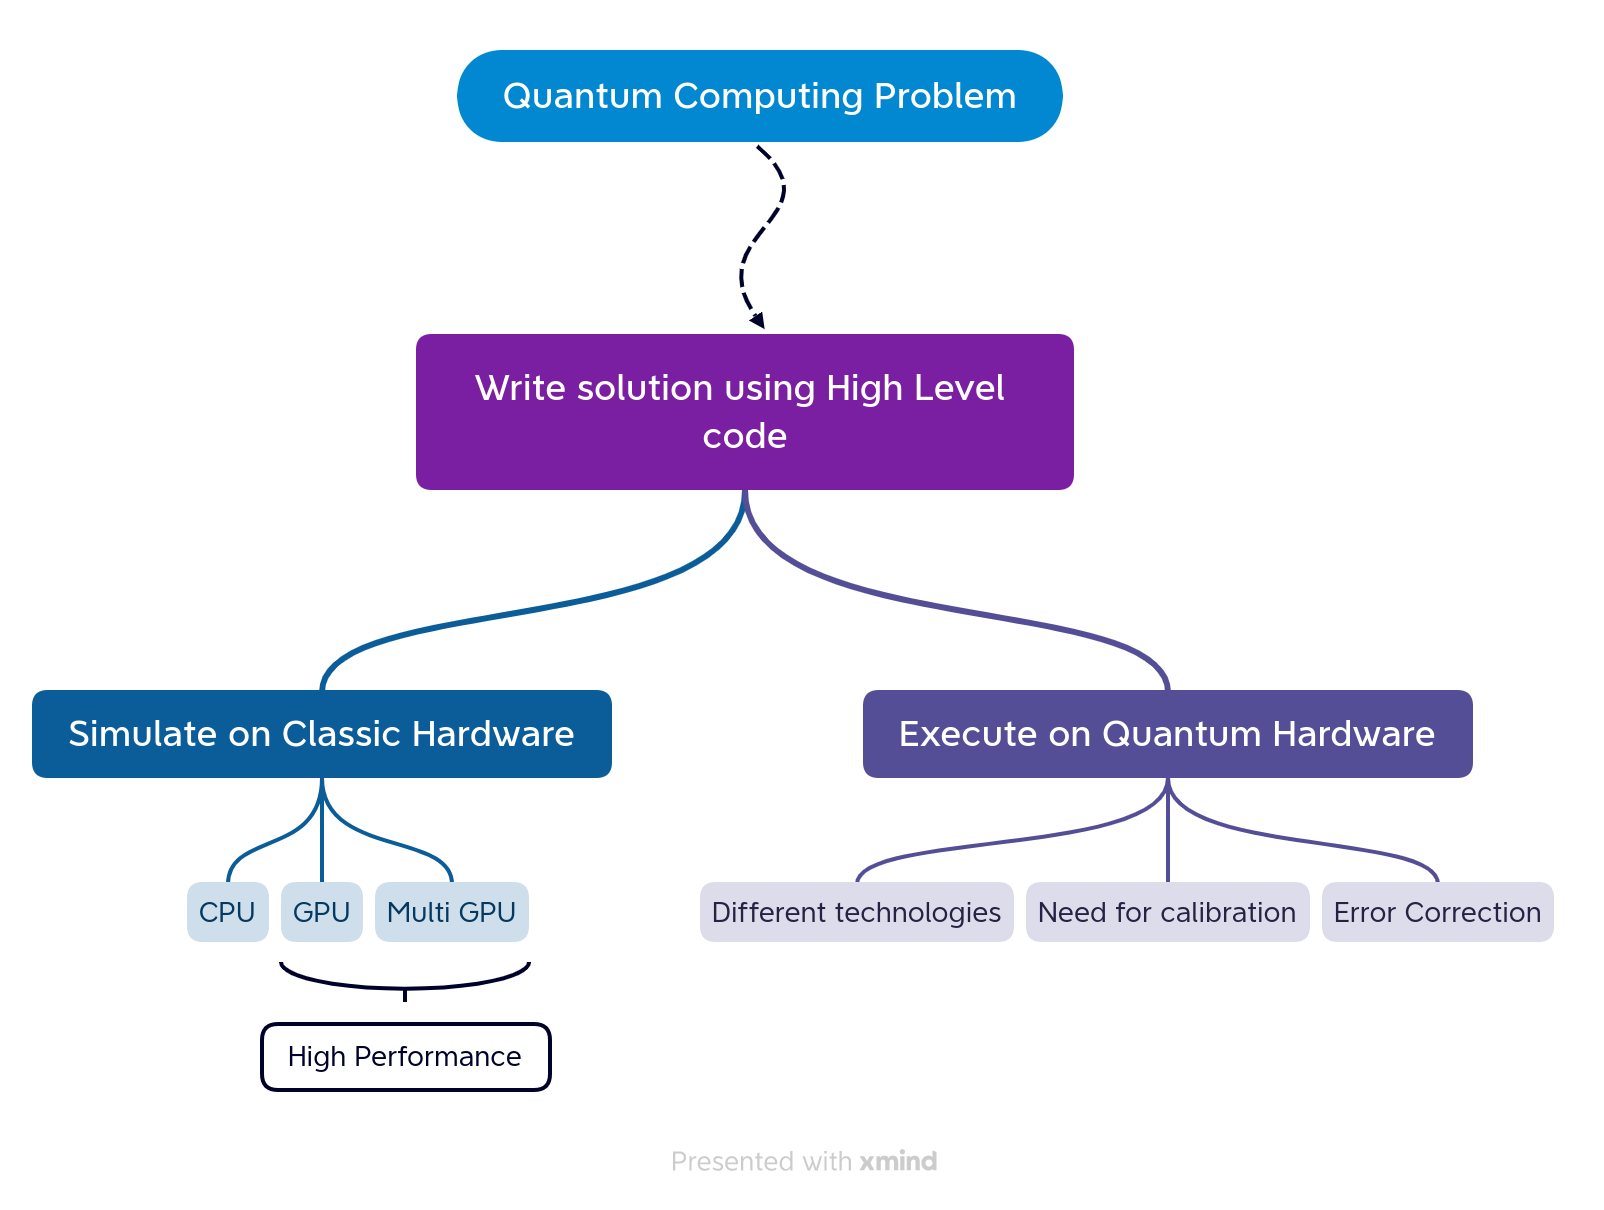
\includegraphics[width=\textwidth]{figures/intro.png}
    \end{figure}
    \centering
    \emph{Is to possible to create from scratch a framework for all of this?}
\end{frame}

% \begin{frame}{User problem}
    
    
% \end{frame}

\section{Introduction on Quantum computing}

\begin{frame}{What is a Qubit?}
    \begin{figure}
        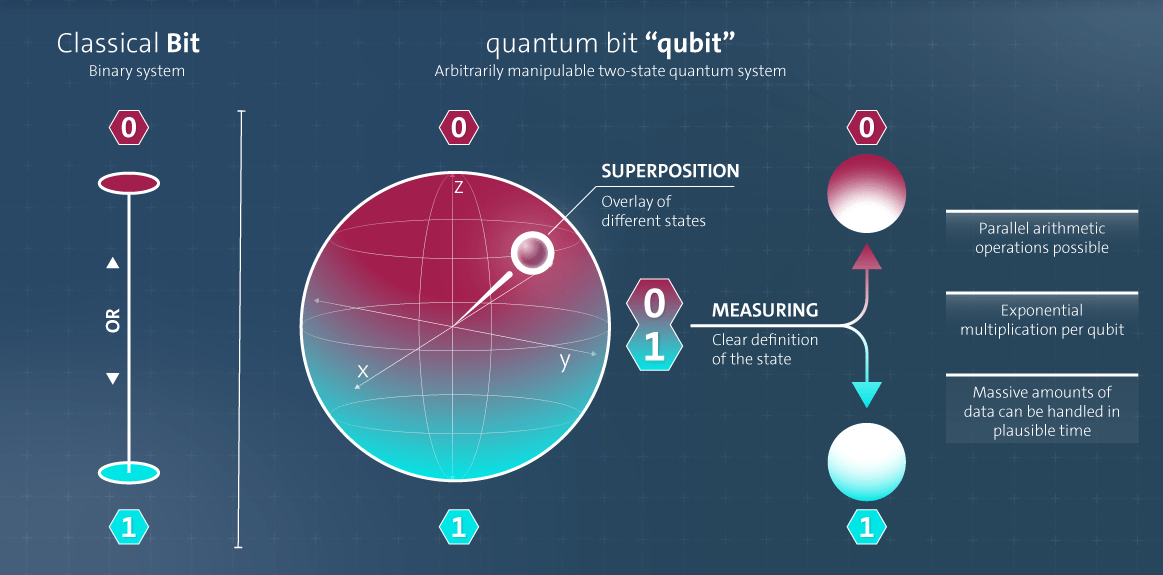
\includegraphics[width= \textwidth]{figures/qubits.png}
    \end{figure}
    \vspace{-0.3cm}
    \begin{tcolorbox}[title=Qubit]
        A qubit is a two state quantum system
        $$ \ket{\psi} = \alpha \ket{0} + \beta \ket{1}  \ ,$$
        where $\alpha$ and $\beta$ are complex numbers such that $|\alpha|^2 + |\beta^2|$ = 1 .
    \end{tcolorbox}
\end{frame}


\begin{frame}{Quantum circuits}
    According to Quantum Mechanics (QM) a state $\psi$ evolves through {\color{blue} unitary} operators $U_i$
    $$ \ket{\psi} \rightarrow \ket{\psi '} = U_2 U_1 \ket{\psi} $$
    In the gates-based model we obtain a circuit:
    $$
    \begin{quantikz}
        \lstick{$\ket{\psi}$} & \qw & \gate{U_1} & \qw &  \gate{U_2} &\qw
        & \rstick{$\ket{\psi '}$} \qw
        \end{quantikz}
        $$
        which we call {\color{red} quantum circuit.}

    With multiple qubits we get the following:
        $$
    \begin{quantikz}
        \lstick[wires=3]{$\ket{\phi}$}
         & \gate{H} & \gate{R_y} & \gate{R_z} & \meter{} & \qw \\
         & \gate{H} & \gate{R_y} & \gate{R_z} &  \meter{} & \qw \\
         & \gate{H} & \gate{R_y} & \gate{R_z} &  \meter{} & \qw
        \end{quantikz}
    $$
    A $n$ qubits system is described by a vector state $\ket{\phi}$ with { \color{red} $2^n$} components.
\end{frame}

% \begin{frame}{Why quantum computing?}
%     Why are we interested in quantum computing?
%     \begin{itemize}
%         \item Analize quantum system using quantum devices
%     \end{itemize}
%     \begin{itemize}
%         \item 
%     \end{itemize}
% \end{frame}

% \begin{frame}
%     \includemovie{3cm}{3cm}{figures/puv1Q.gif}
% \end{frame}

\section{How can we implement physical qubits?}

\begin{frame}{Quantum technologies}
    \begin{figure}
        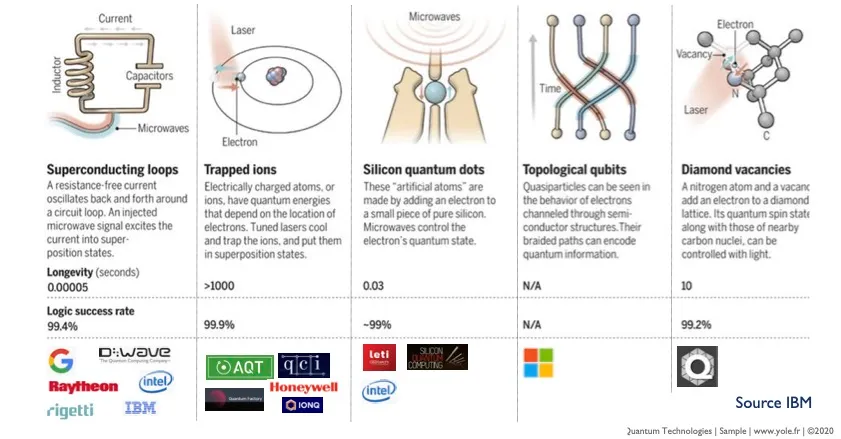
\includegraphics[width=\textwidth]{figures/quantum_technologies.png}
    \end{figure}
\end{frame}


\section{Introducing Qibo}

\begin{frame}{Qibo}
    Qibo is an \textbf{open-source} full stack API for quantum simulation and quantum hardware control and calibration.
    \begin{figure}
        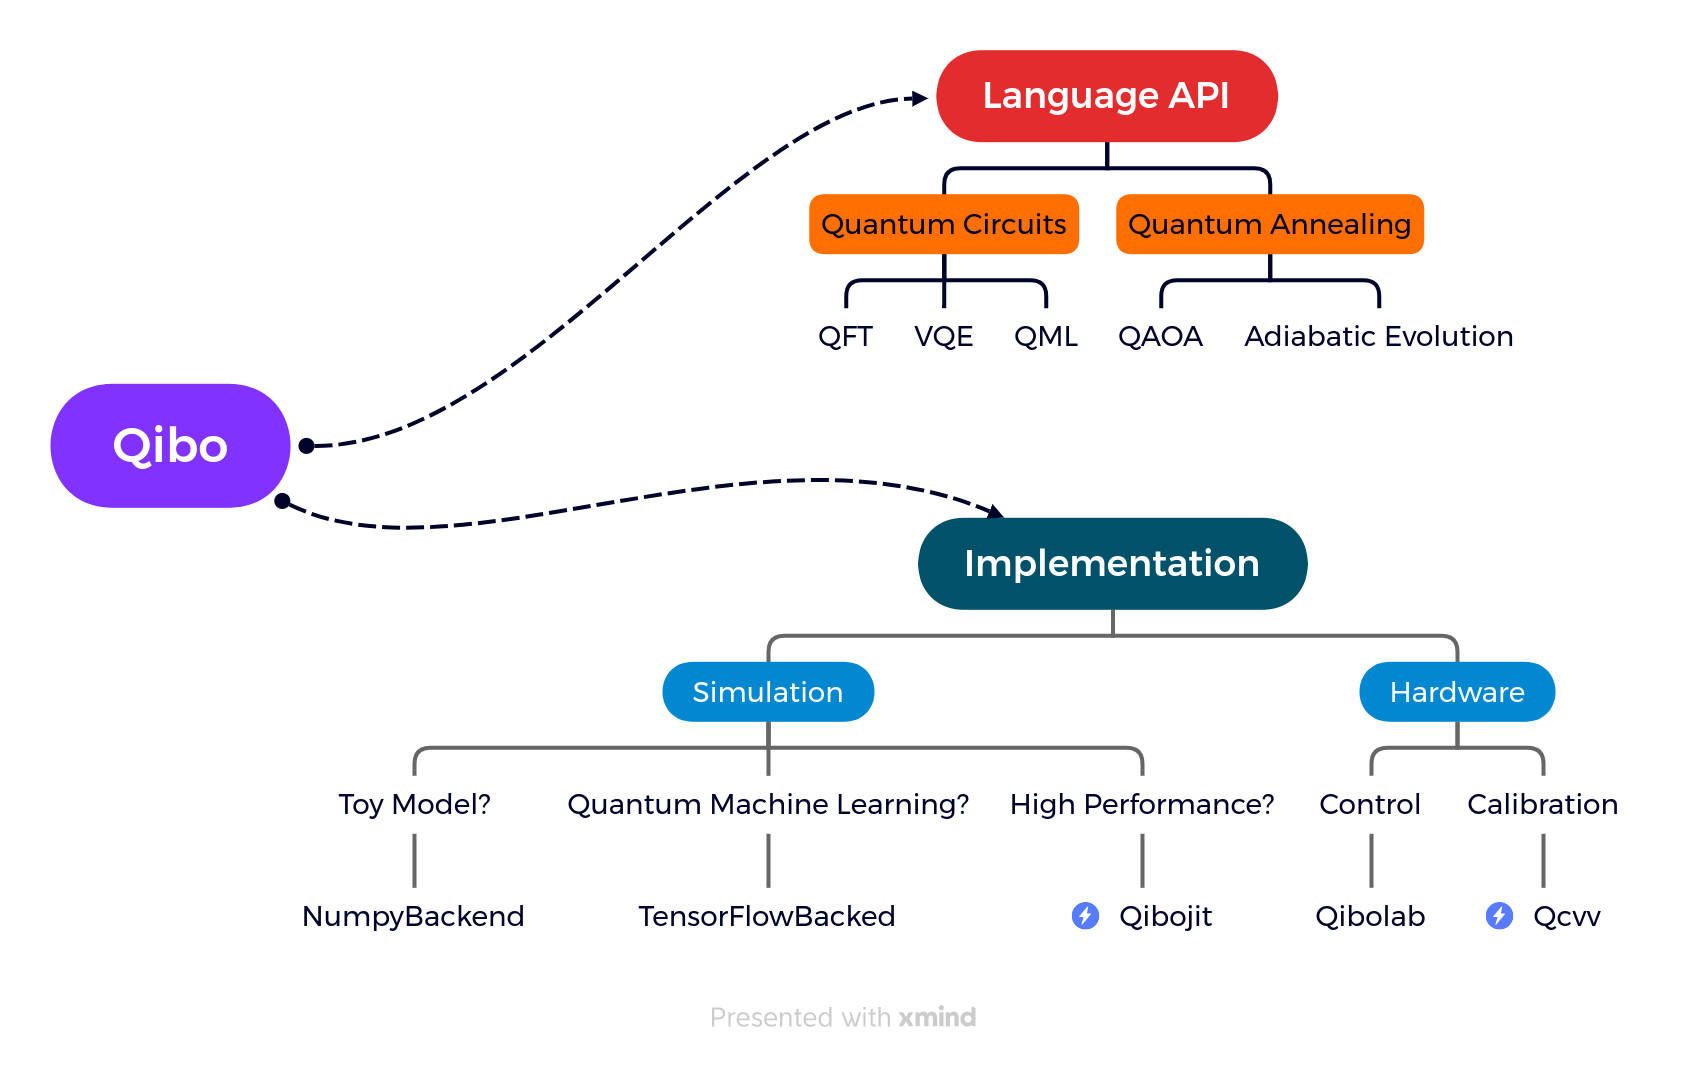
\includegraphics[width= \textwidth]{figures/Qibo.png}
    \end{figure}
    
\end{frame}

% \begin{frame}{A modular framework for quantum computing}
%     \begin{figure}
%         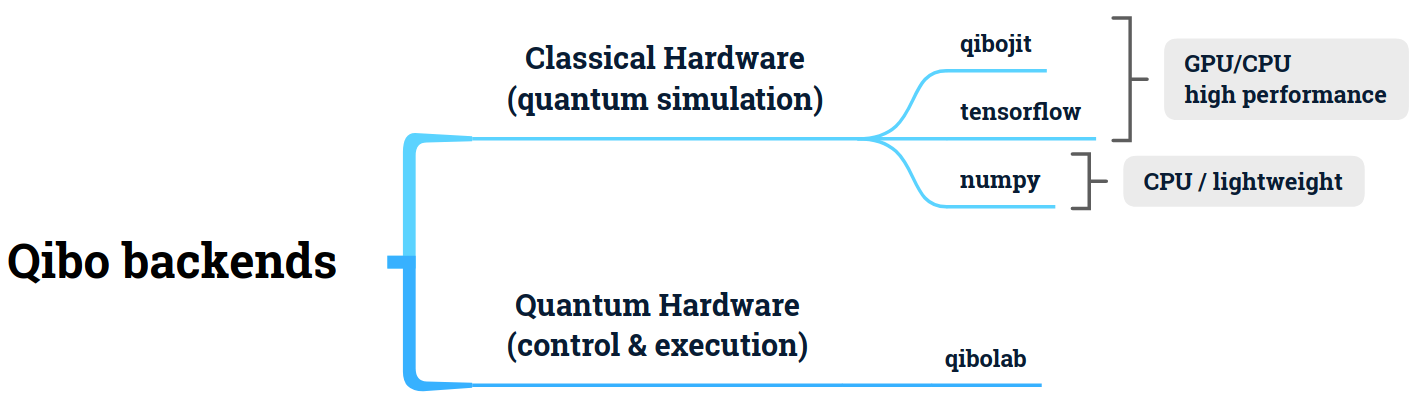
\includegraphics[width= \textwidth]{figures/backends.png}
%     \end{figure}
% \end{frame}

\begin{frame}{Introducing Qibojit}
    Matrix multiplication to simulate circuits:

    \begin{equation*}\label{eq:gateapplication}
        \psi'(\sigma_1, \ldots, \sigma_n) = \sum _{\boldsymbol{\tau'}} G(\boldsymbol{\tau}, \boldsymbol{\tau'})\psi(\sigma_1,\ldots,\boldsymbol{\tau'},\ldots,\sigma_n) \ .
    \end{equation*}

    
    
    { \color{red} \faClose}  Number of operations scales { \color{red} exponentially} with the number of qubits!
   
    We need more sophisticated backends to perform simulation:
    \begin{itemize}
        \item[{ \color{red} \faClose}] \texttt{NumpyBackend} : { \color{blue} Numpy} tensors and primitives
        \item[{ \color{red} \faClose}] \texttt{TensorFlowBackend} : { \color{orange} Tensorflow} tensors and primitives
        \item[{ \color{green} \faCheck}] \texttt{QibojitBackend} : Just-In-time
        \item[]     \begin{itemize}
            \item[\faCode] CPU : { \color{blue} Numpy} tensor + custom operations with {\color{cyan} Numba JIT}
            \item[\faCode] GPU(S) : {\color{teal} Cupy} tensors + custom operations using
            \begin{itemize}
                \item  {\color{teal} Cupy JIT} Raw kernels
                \item  {\color{green} NVIDIA cuQuantum}  API
            \end{itemize} 
        \end{itemize}
    \end{itemize}

    Paper published on Quantum: \url{https://quantum-journal.org/papers/q-2022-09-22-814/}

    
\end{frame}

\begin{frame}[fragile]{Qibojit - Example}

    \begin{columns}
        \begin{column}{0.7\textwidth}
            \hspace{1cm}
            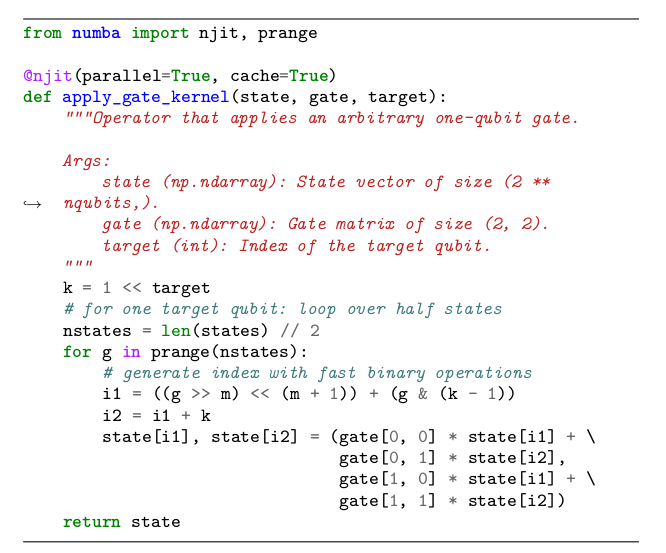
\includegraphics[width = 0.8\textwidth]{figures/circuit.png}
        \end{column}

        \begin{column}{0.6\textwidth}
            To further speed up:
            \begin{itemize}
                \item \emph{in-place updates}
                \item exploit sparsity of matrices
                \item specialized operators for:
                \begin{itemize}
                    \item single qubit gate: X, Y Z
                    \item two qubit gates: SWAP
                \end{itemize}
            \end{itemize}
        \end{column}
    \end{columns}

    
\end{frame}

\begin{frame}{Benchmarks}
    \begin{figure}
        % 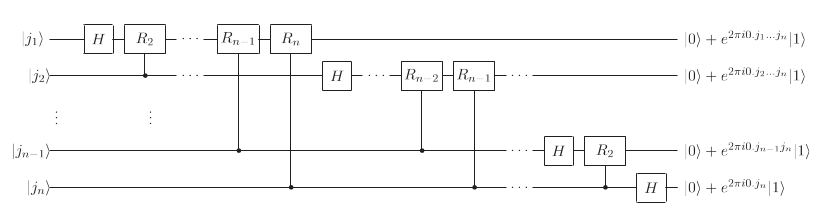
\includegraphics[width=0.8 \textwidth]{figures/qft.png}
        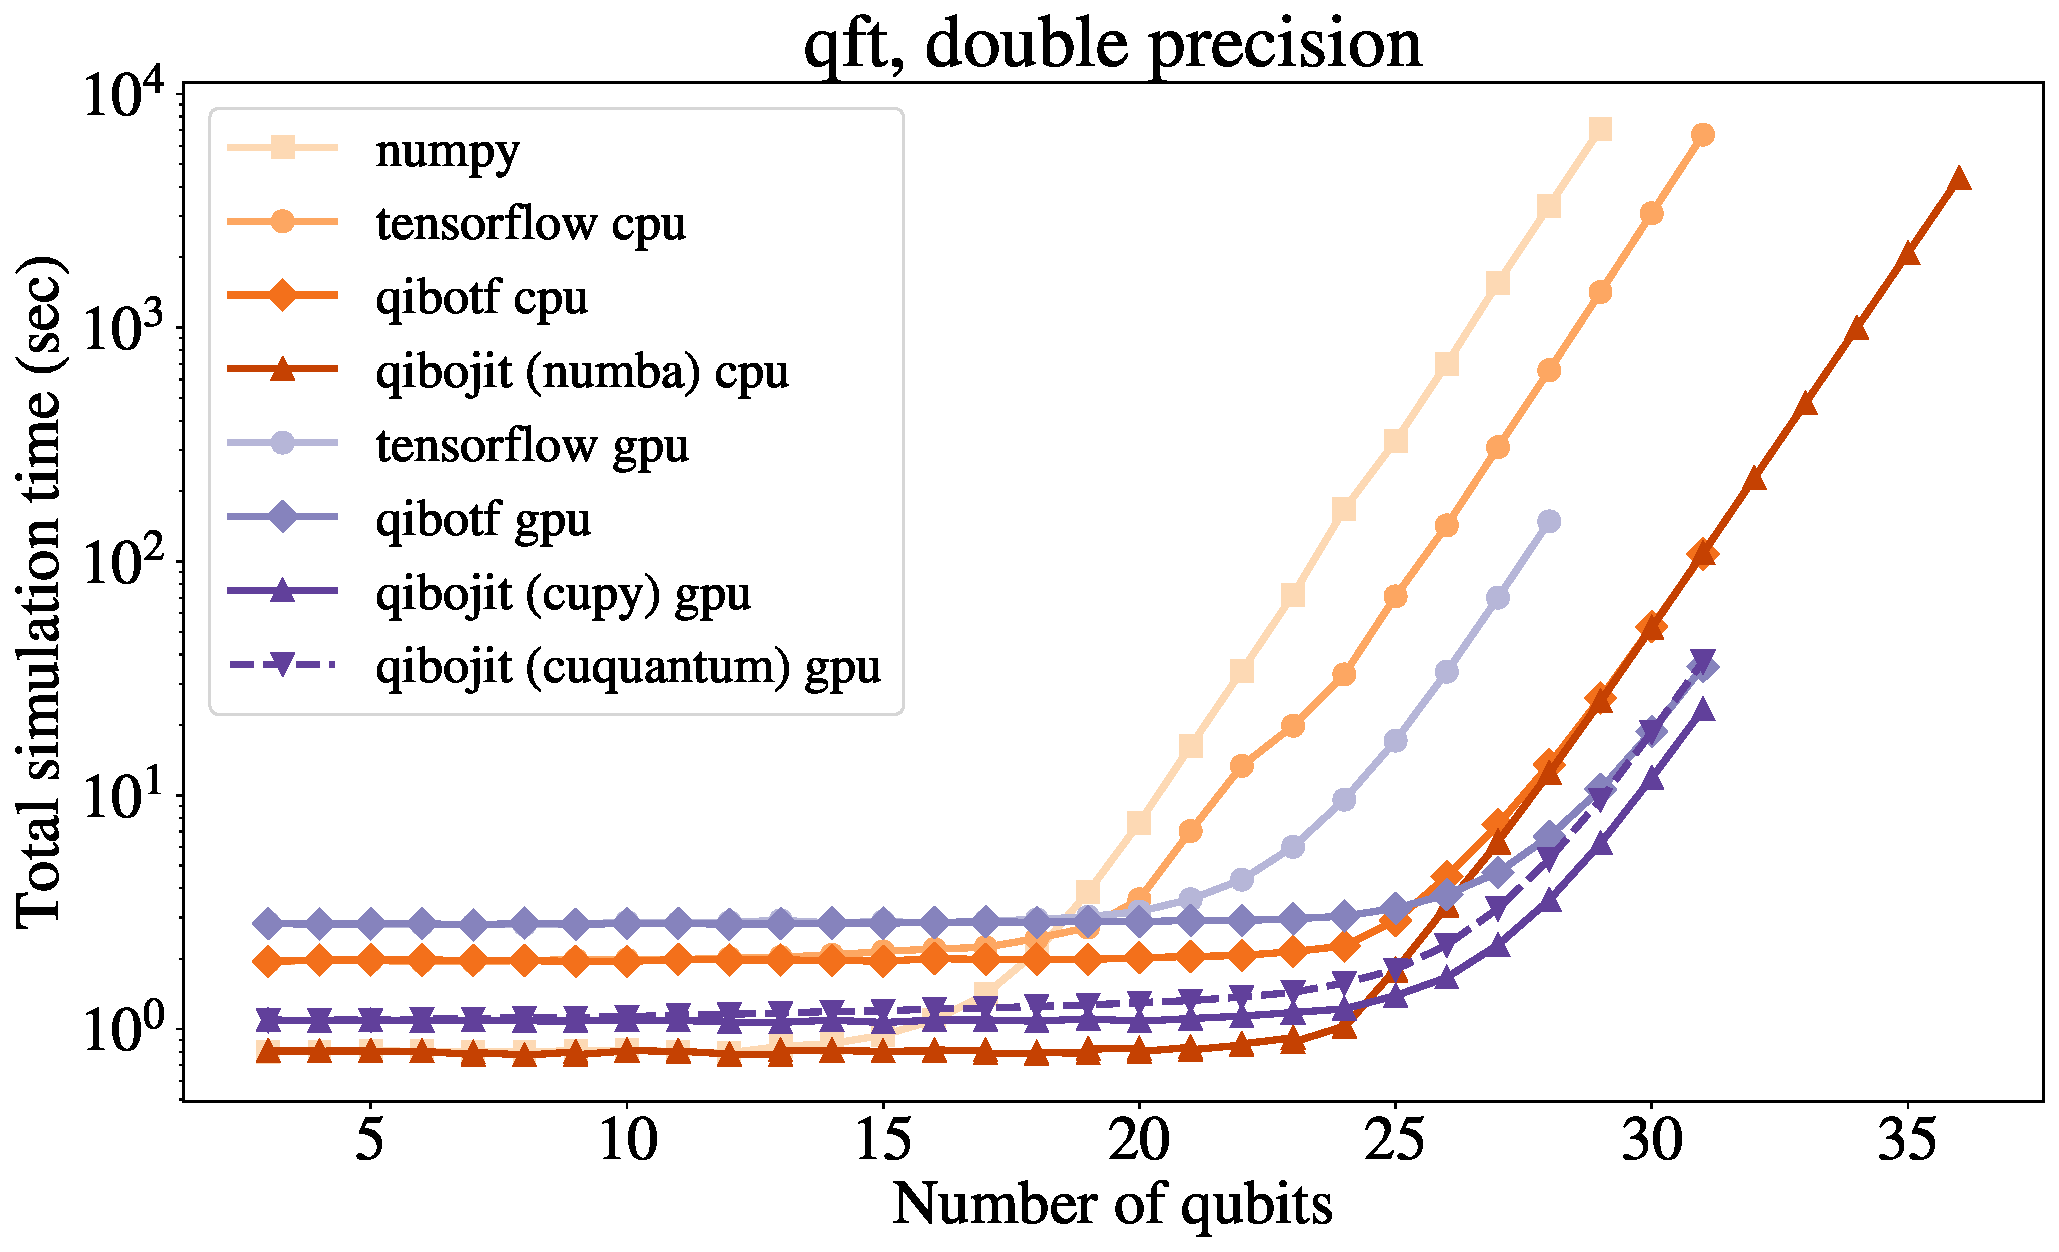
\includegraphics[width=0.8 \textwidth]{figures/qibo_scaling_qft_total_simulation_time_double.pdf} 
    \end{figure}
    Benchmark library: \url{https://github.com/qiboteam/qibojit-benchmarks}
\end{frame}

\begin{frame}{Benchmarks}
    \begin{columns}
        \begin{column}{0.8 \textwidth}

            % \begin{figure}[ht]
            %     \fbox{\begin{minipage}[t]{0.8 \textwidth}
            %       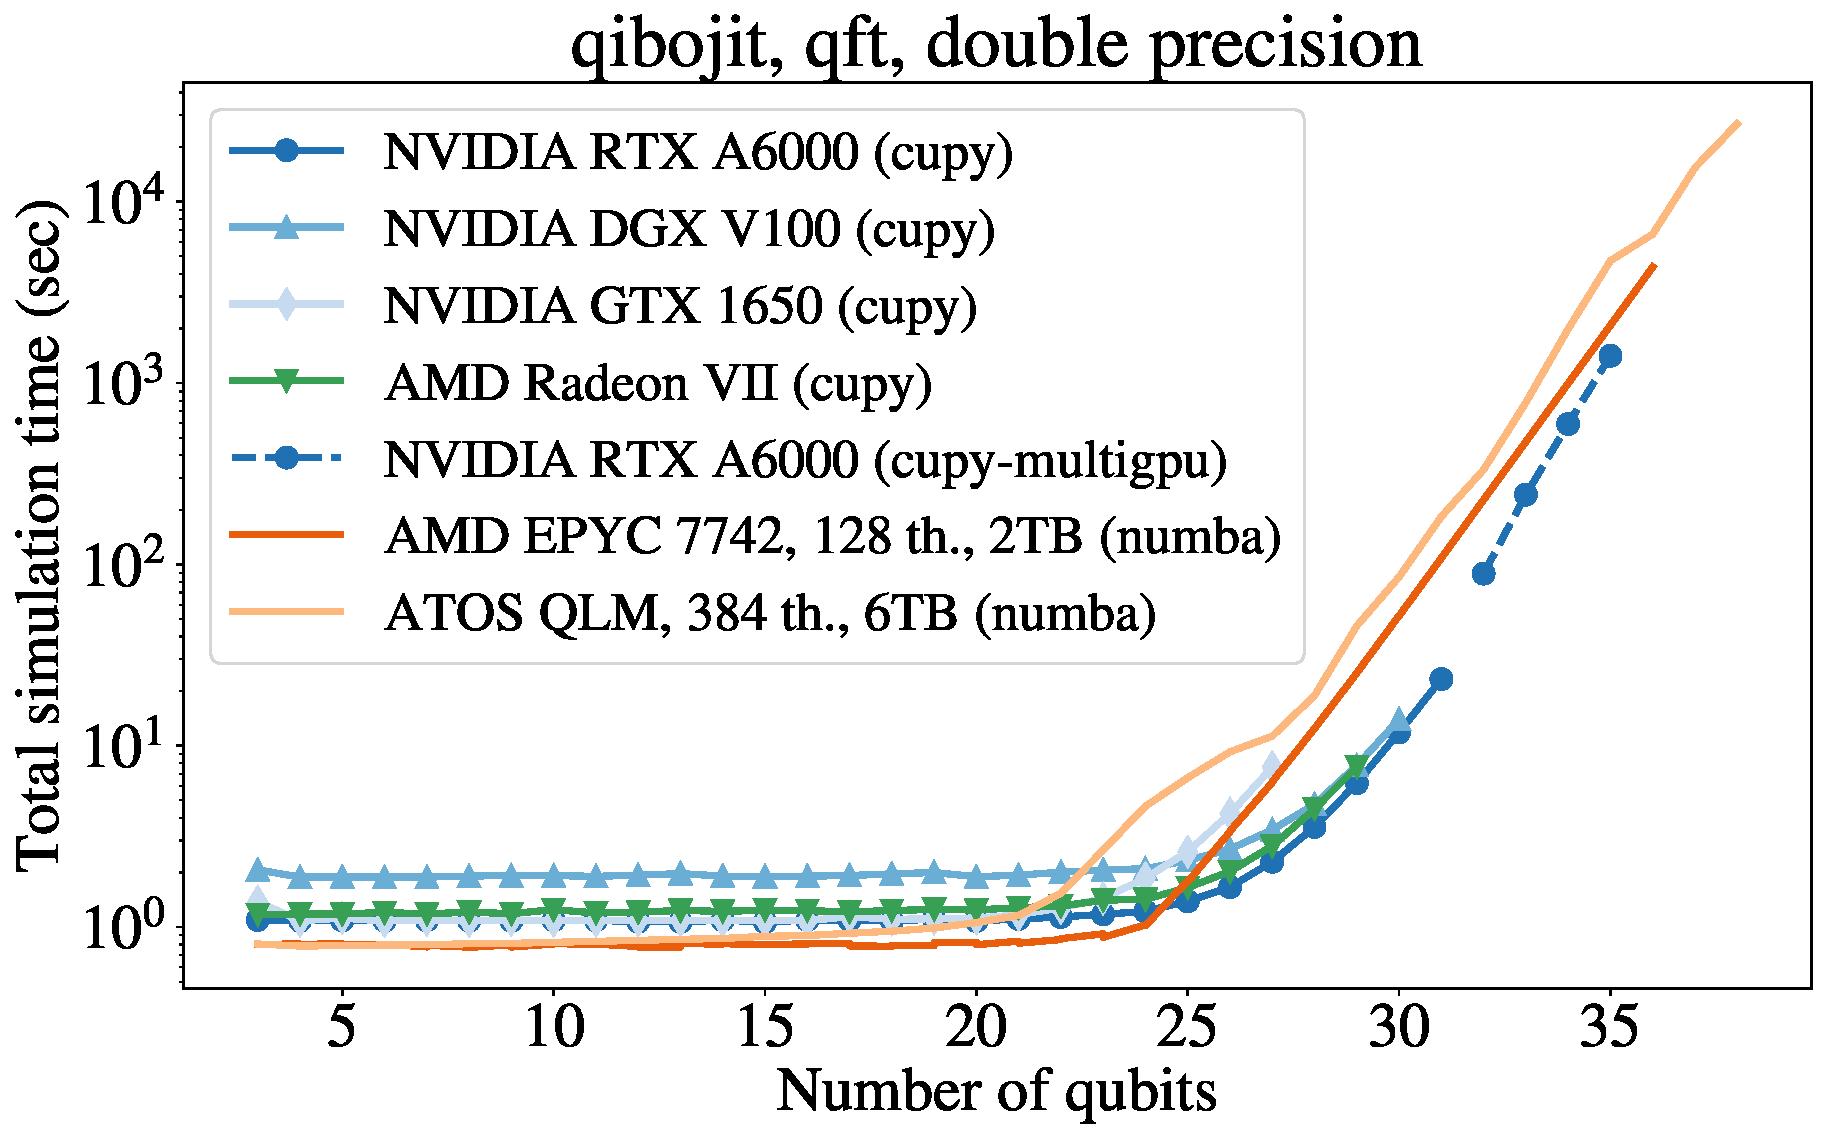
\includegraphics[width=0.8 \textwidth]{figures/devices_qft_total_simulation_time_double.pdf}
            %     \end{minipage}}
            %     \hfill
            %     \fbox{\begin{minipage}[t]{0.8 \textwidth}
            %       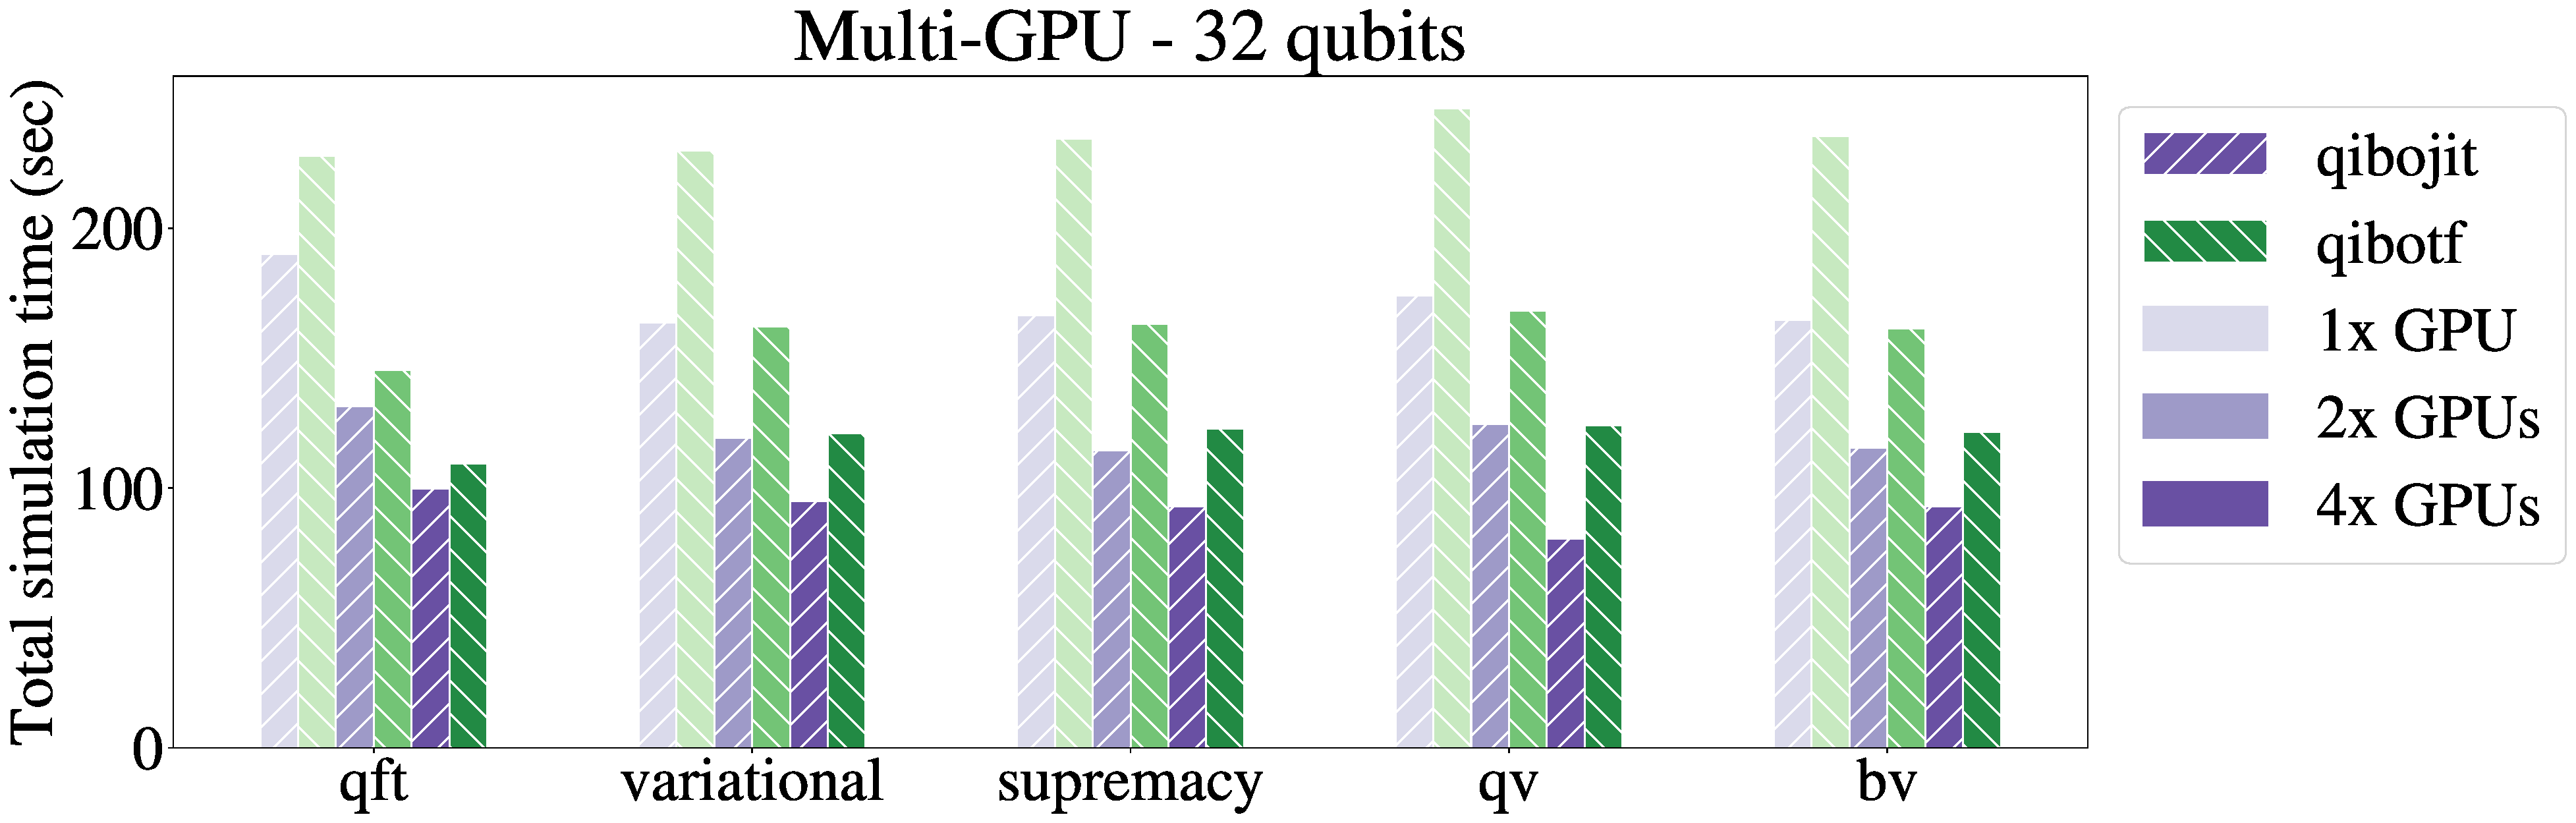
\includegraphics[width=0.8 \textwidth]{figures/multigpu_32qubits_total_simulation_time_double.pdf}
            %     \end{minipage}}
            %   \end{figure}
            \begin{figure}
            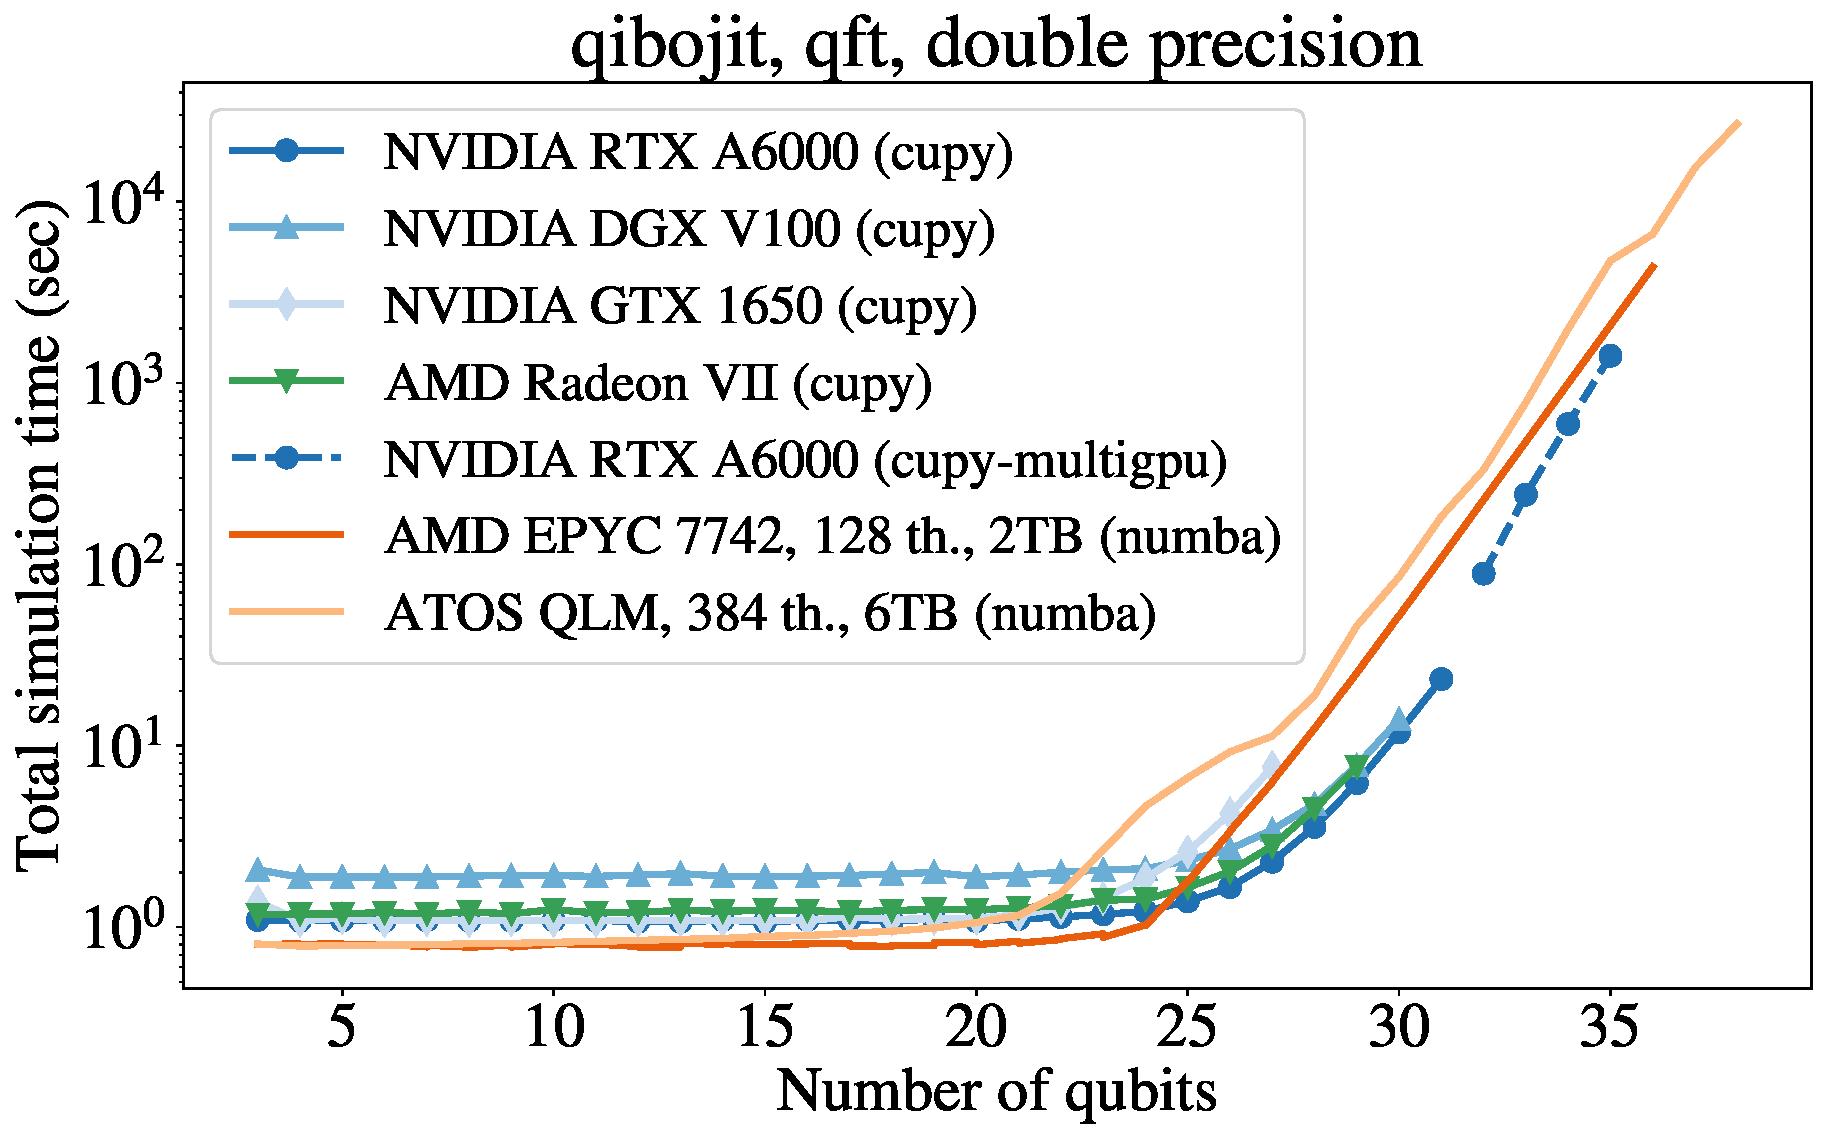
\includegraphics[width=0.8 \textwidth]{figures/devices_qft_total_simulation_time_double.pdf}
            \hspace{0.5cm}

            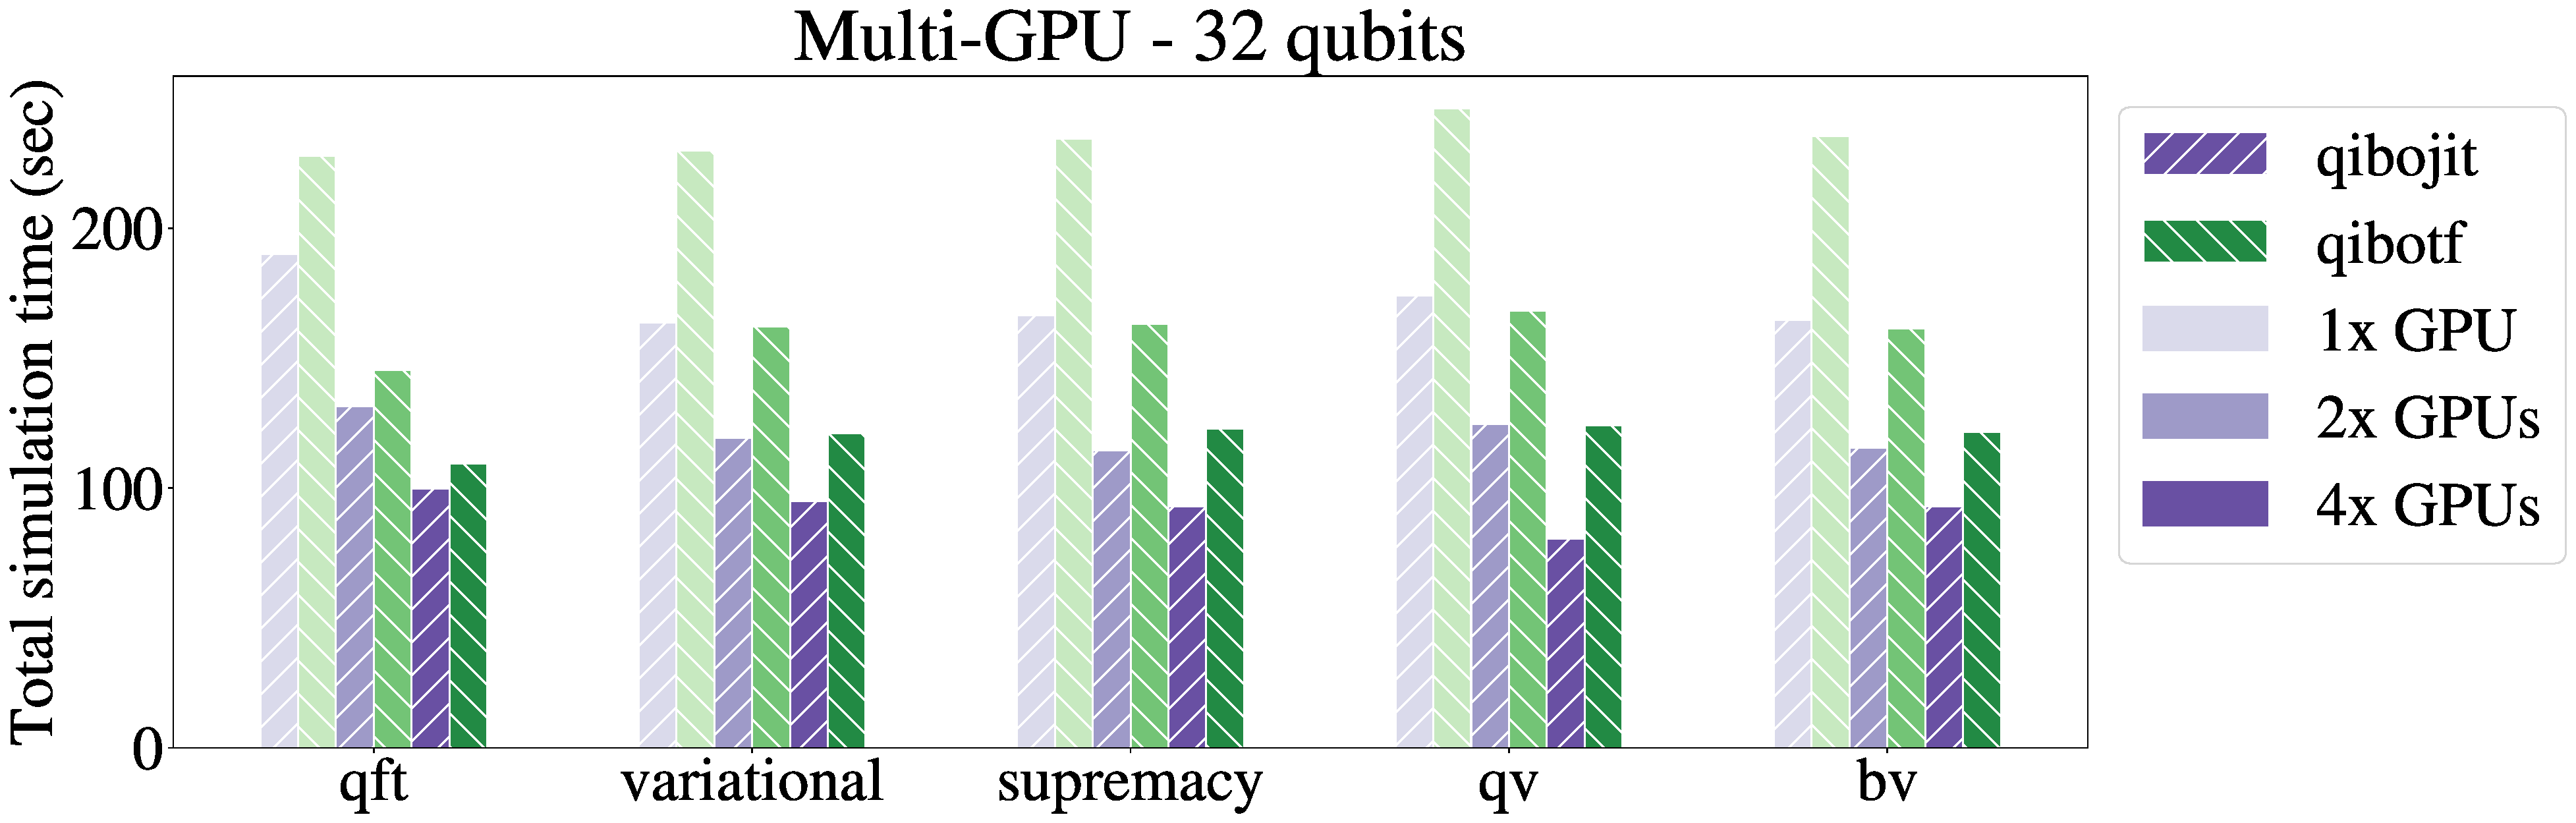
\includegraphics[width=0.8 \textwidth]{figures/multigpu_32qubits_total_simulation_time_double.pdf}
            \end{figure}
        \end{column}
        \hspace{-1cm}
        \begin{column}{0.4 \textwidth}
            \vspace{-1cm}

            Qibojit features
            \begin{itemize}
                \item Support for CPU, GPU and multi-GPU
                \item NVIDIA and AMD (ROCm) GPUs
                \item Reduced memory footprint
            \end{itemize}
        \end{column}
    \end{columns}
    Benchmark library: \url{https://github.com/qiboteam/qibojit-benchmarks}
    
\end{frame}


\begin{frame}{How does Qibo perform against the other libraries?}
    \begin{figure}
        \centering
        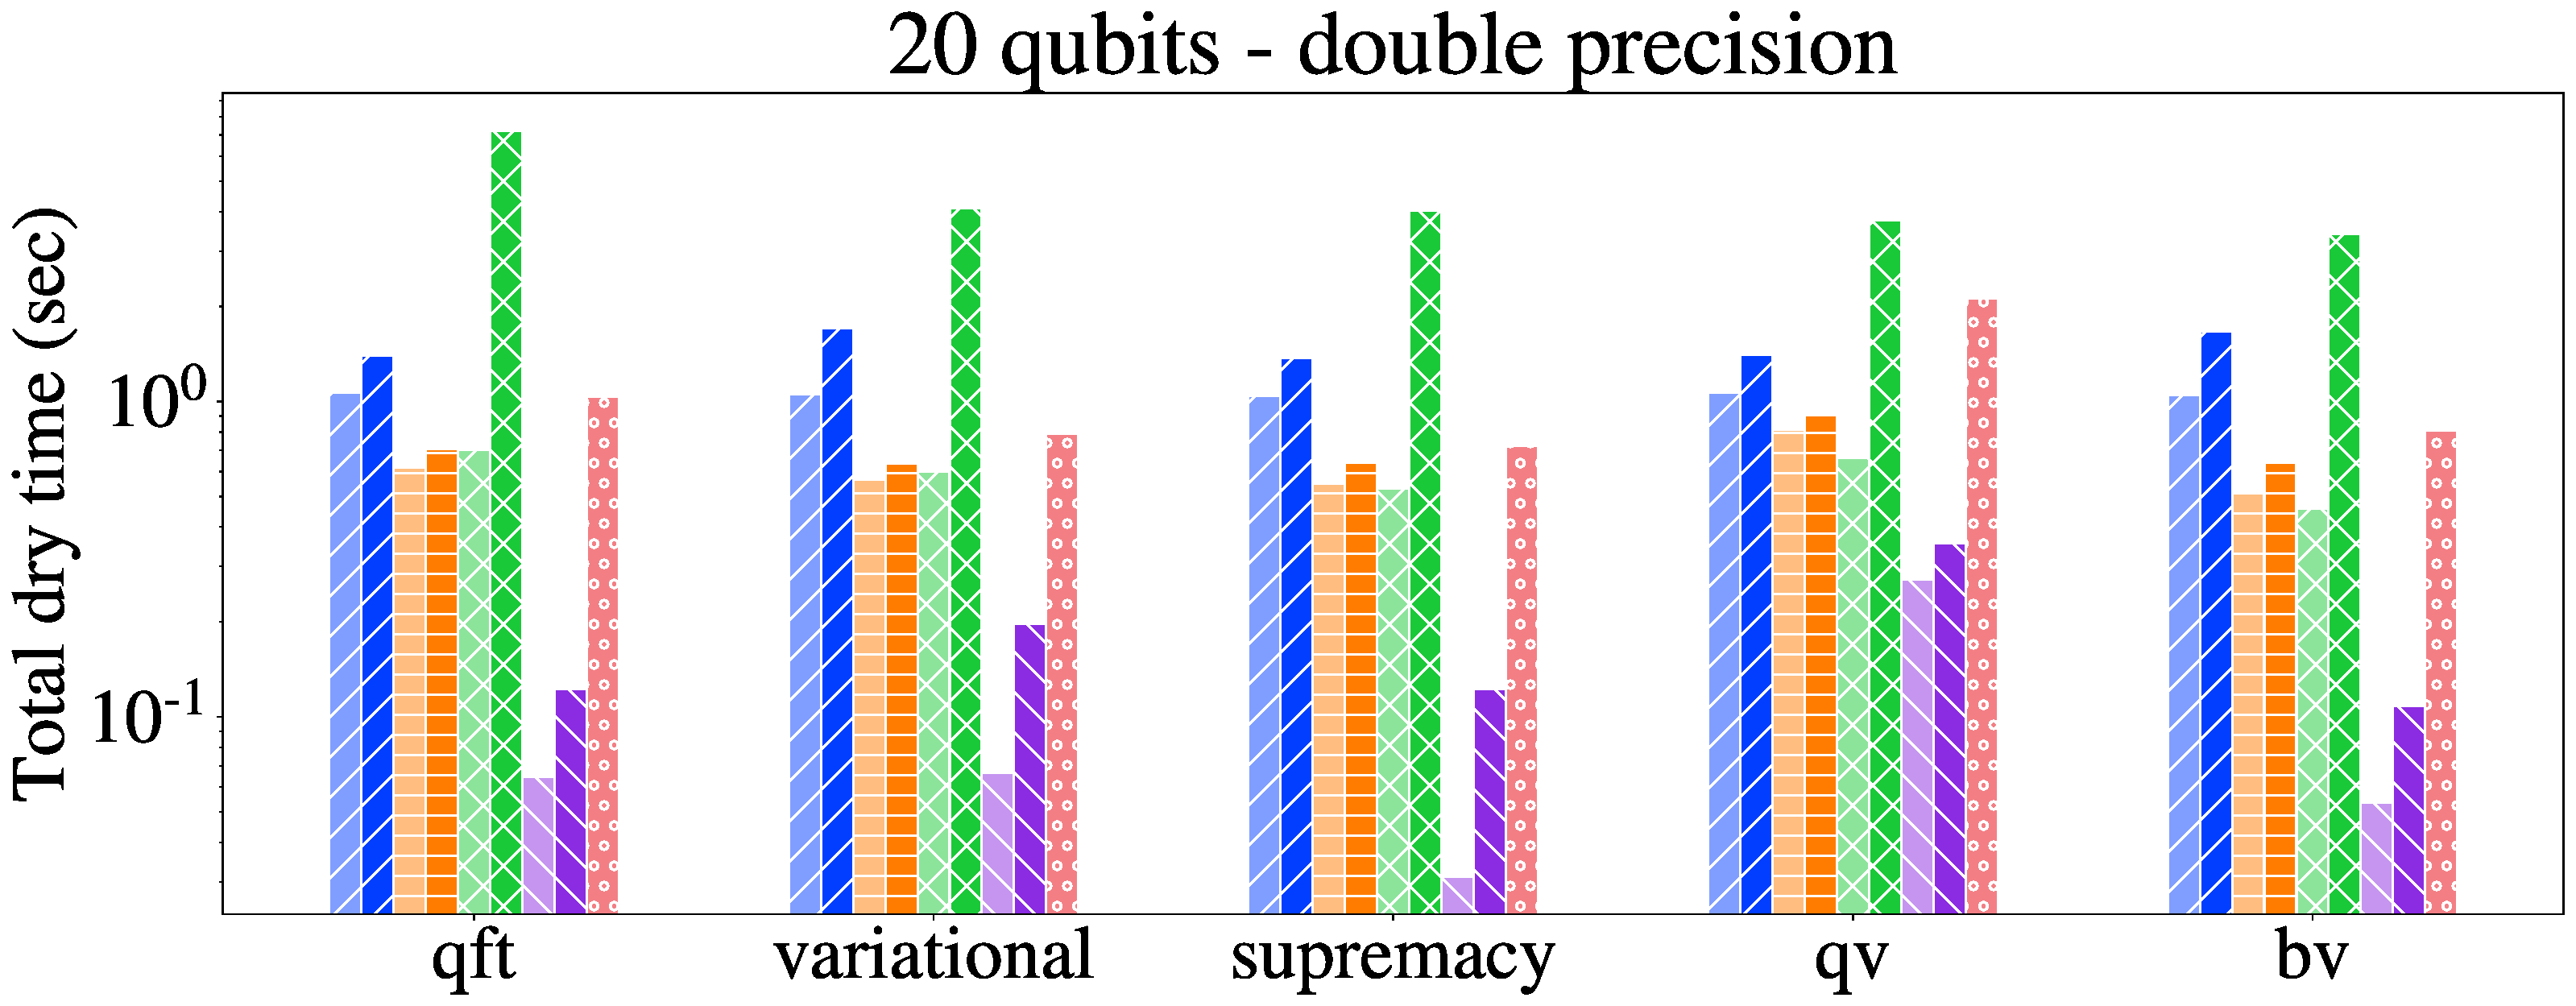
\includegraphics[height=0.4\textheight]{figures/libraries_double_20qubits_total_dry_time.pdf}
        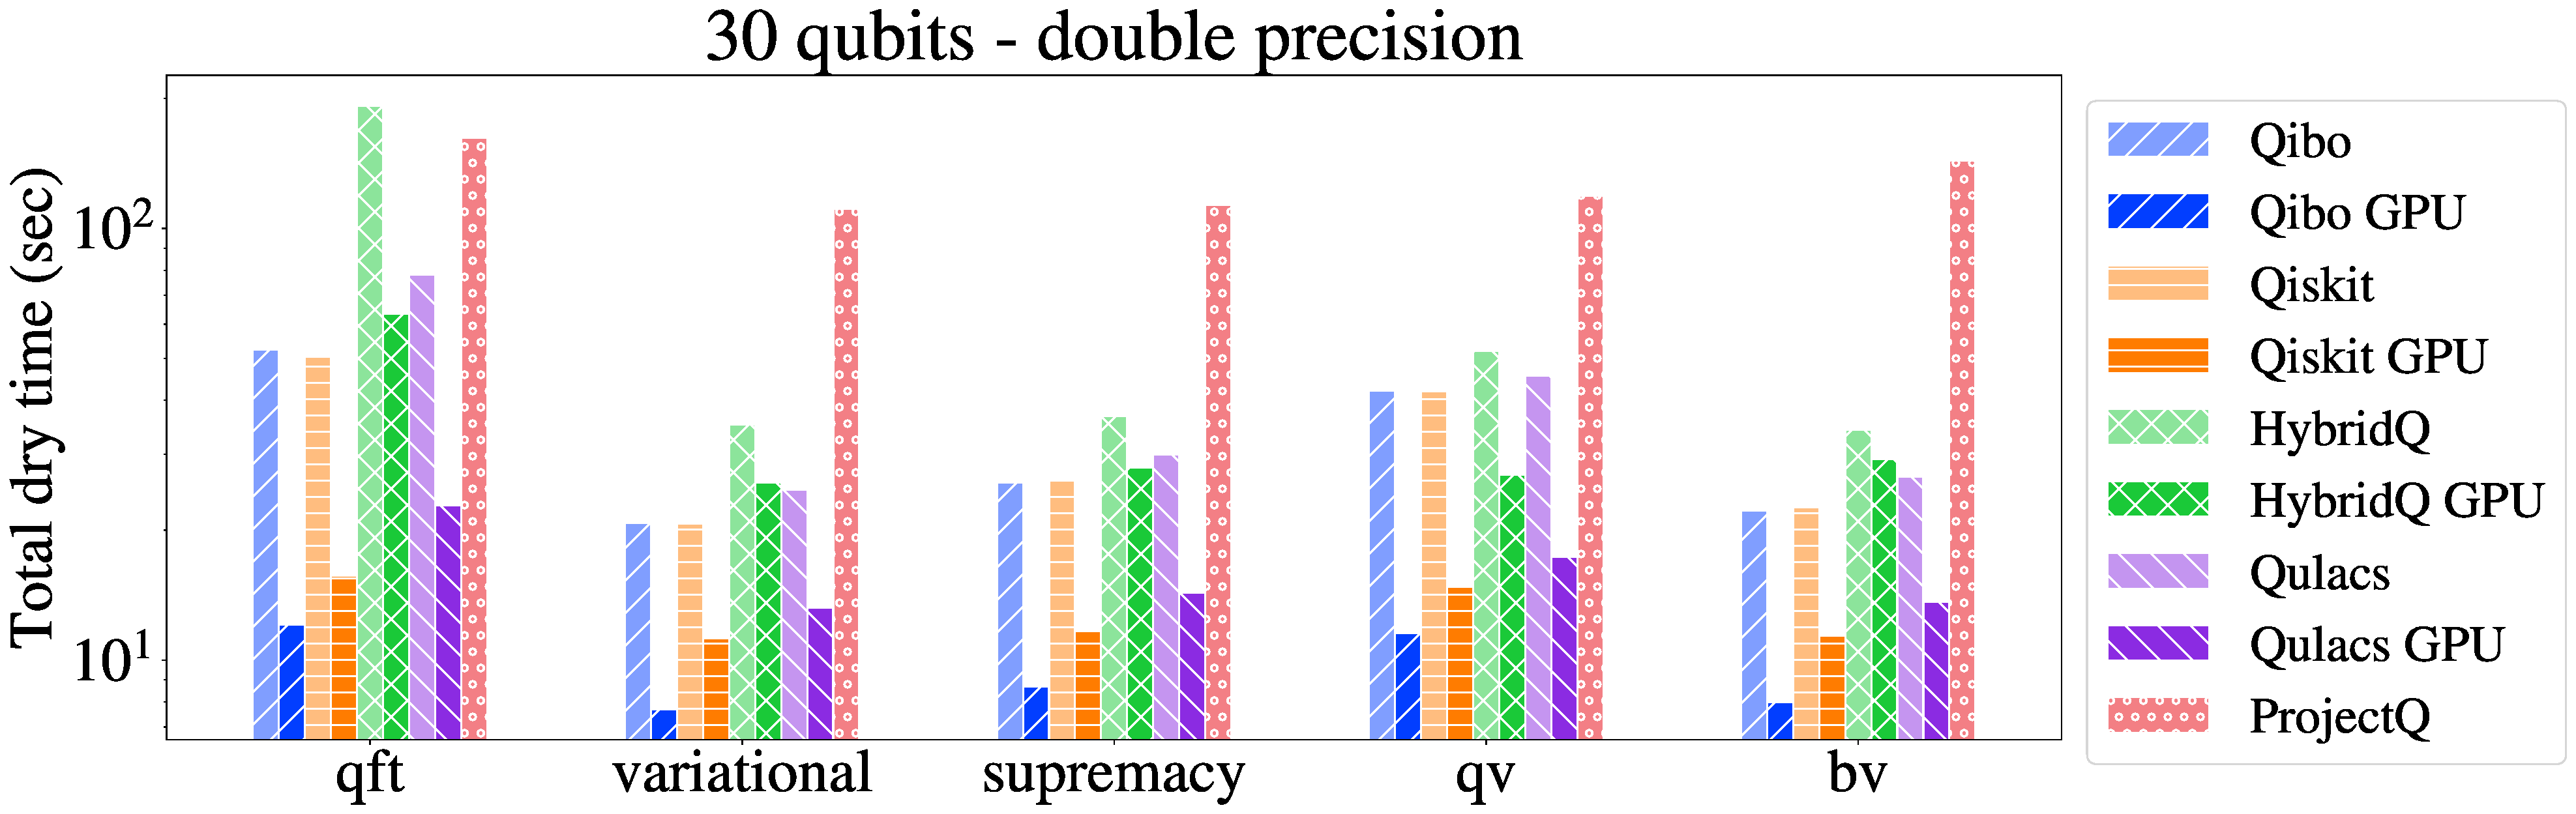
\includegraphics[height=0.31\textheight]{figures/libraries_double_30qubits_total_dry_time.pdf}
    \end{figure}
    Benchmark library: \url{https://github.com/qiboteam/qibojit-benchmarks}
    
\end{frame}

\section{Hardware control using Qibo}

% \begin{frame}{Hardware control}
%     A quantum computer has many components outside the chip...
%     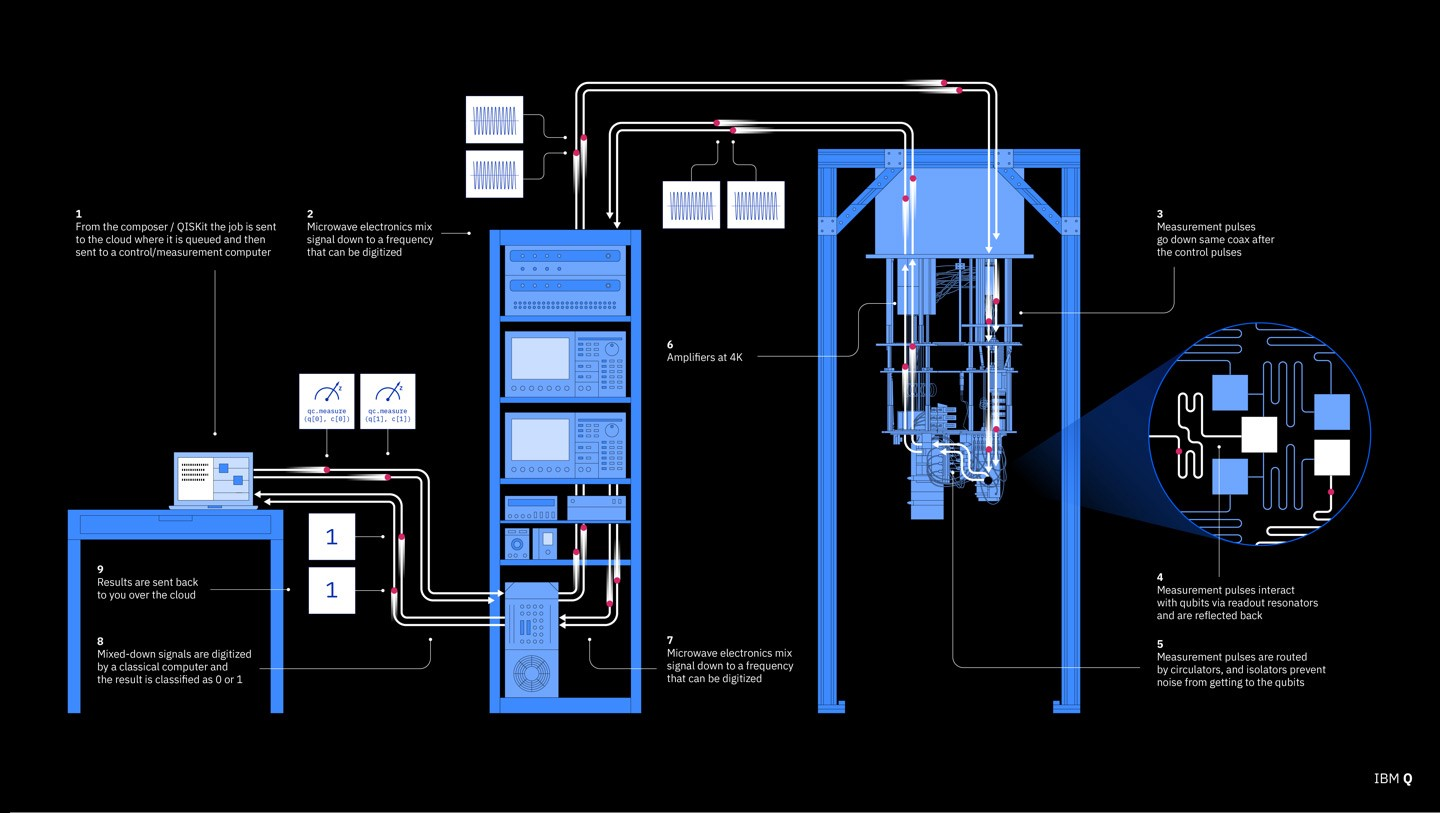
\includegraphics[width = \textwidth]{figures/quantum_computer.jpeg}


    
% \end{frame}

\begin{frame}{Hardware control}
    For superconducting qubits \textbf{gates} are implemented by sending \textbf{pulses}.

    \begin{columns}
        \begin{column}{0.5 \textwidth}
            \begin{figure}
                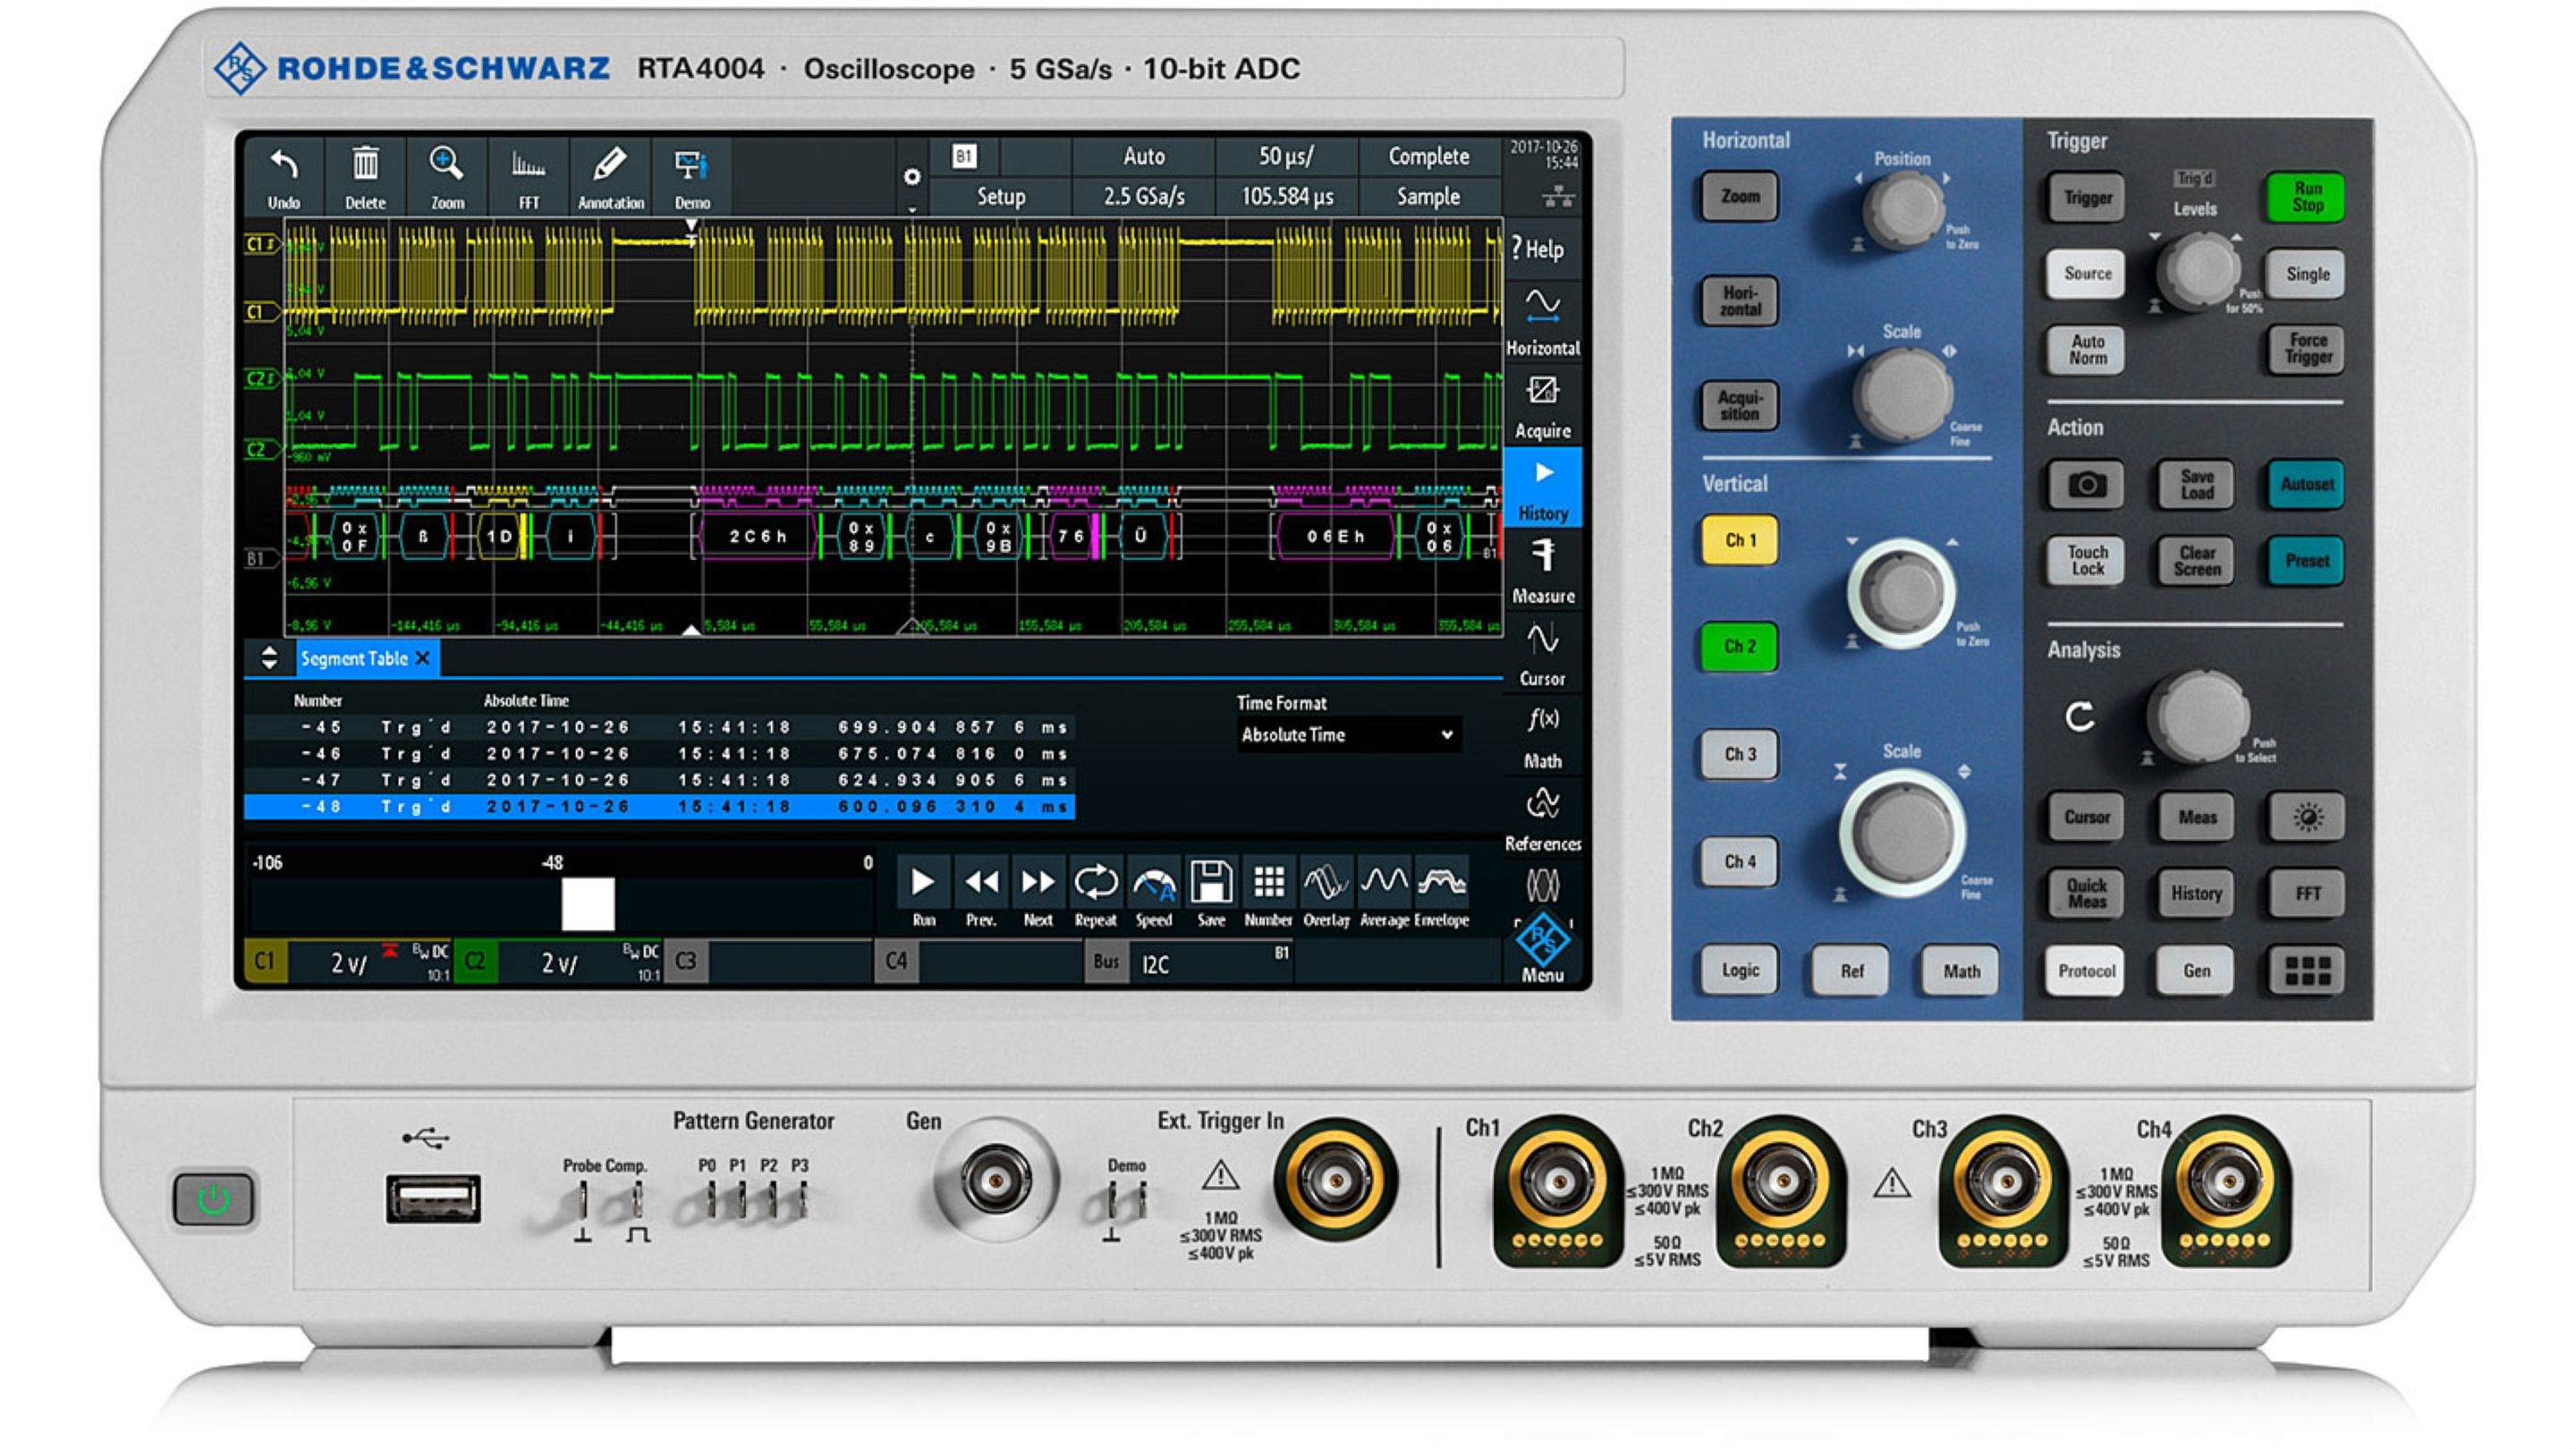
\includegraphics[height = 0.3 \textheight]{figures/rohde.jpg}
                % \caption{Oscilloscope}
            \end{figure}
            
            % \begin{itemize}
            %     \item Wavefunction generators
            %     \item Local oscillators
            %     \item Qblox devices
            %     \item Custom FPGA boards
            %    \end{itemize}
        \end{column}
        \begin{column}{0.5 \textwidth}
            % 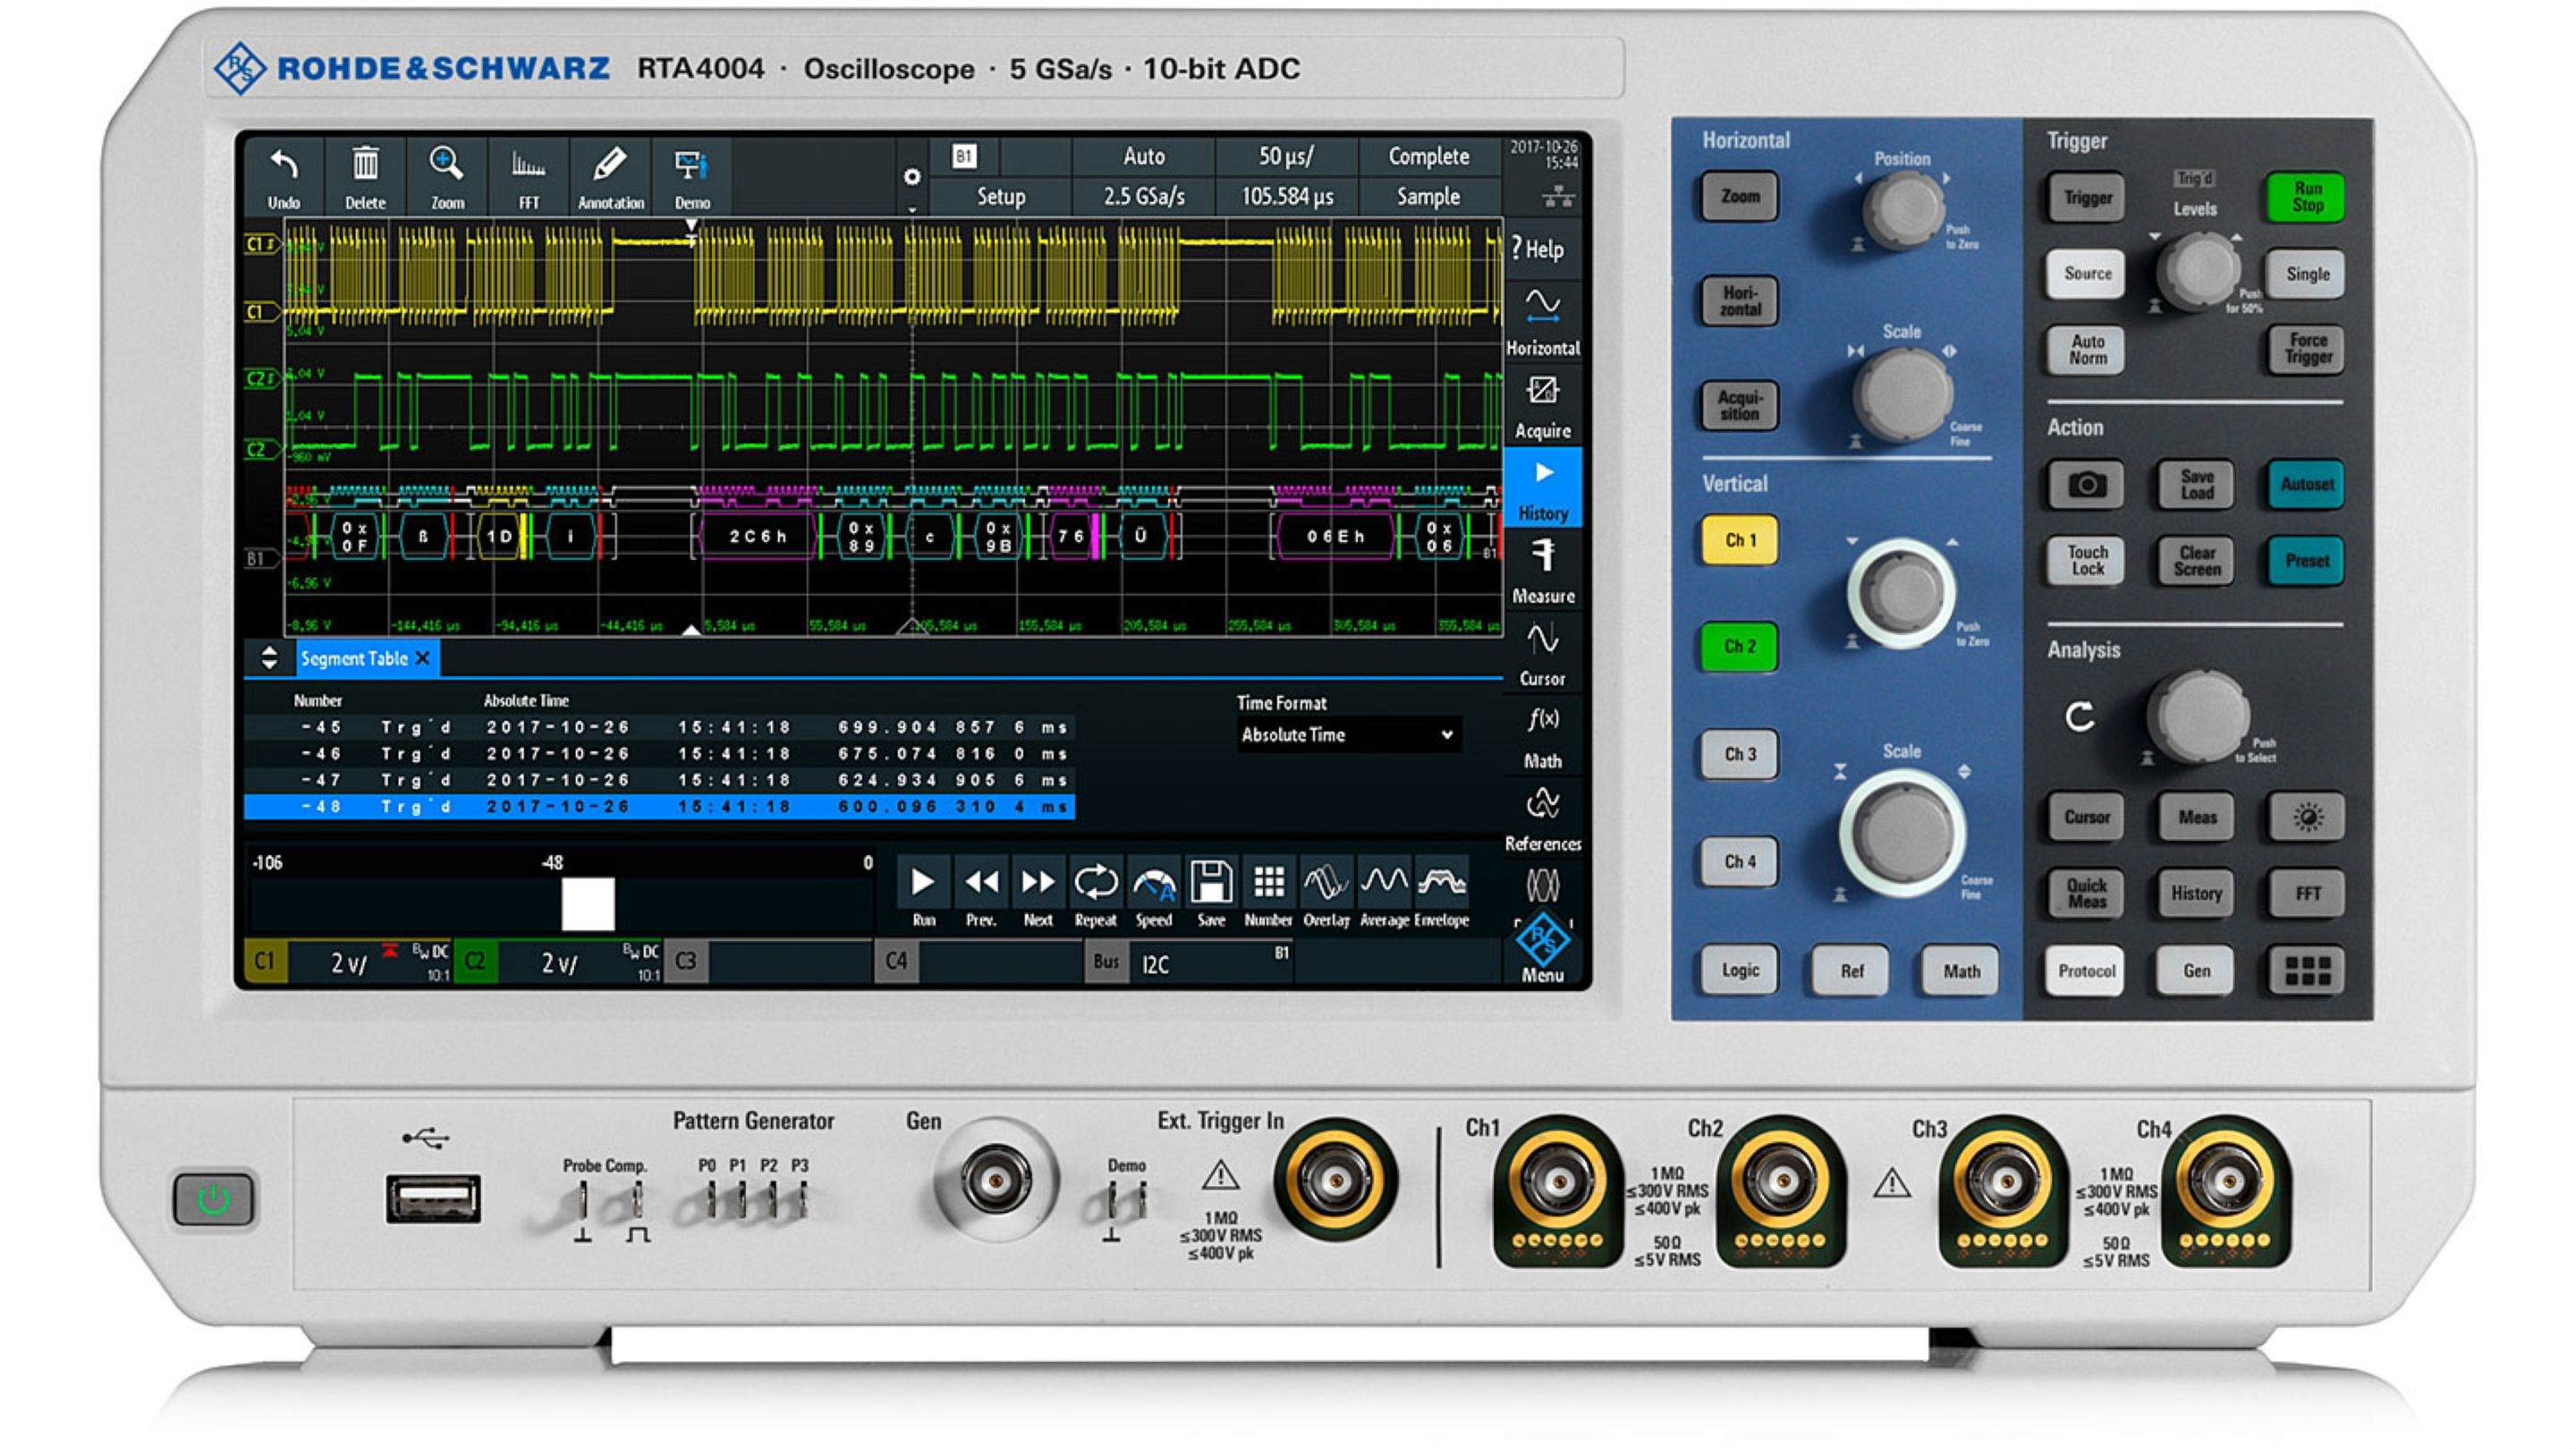
\includegraphics[height = 0.3 \textheight]{figures/rohde.jpg}
            \begin{figure}
                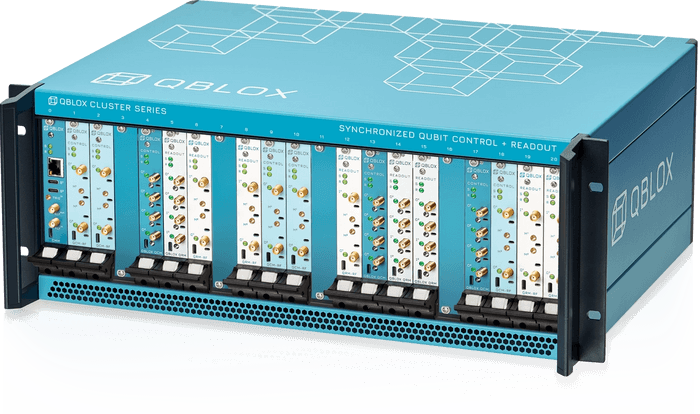
\includegraphics[height = 0.3 \textheight]{figures/qblox.png}
                % \caption{Qblox}
                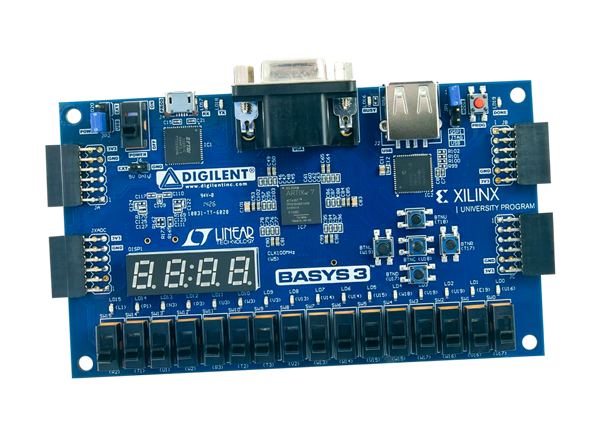
\includegraphics[height = 0.3 \textheight]{figures/fpga.png}
                % \caption{FPGA board}
            \end{figure}
            
        \end{column}
    \end{columns}
  
   We need a framework to control all these devices at the same time.
    
\end{frame}

\begin{frame}{Introducing Qibolab}
    \begin{columns}
        \begin{column}[]{0.5 \textwidth}
            \begin{figure}
                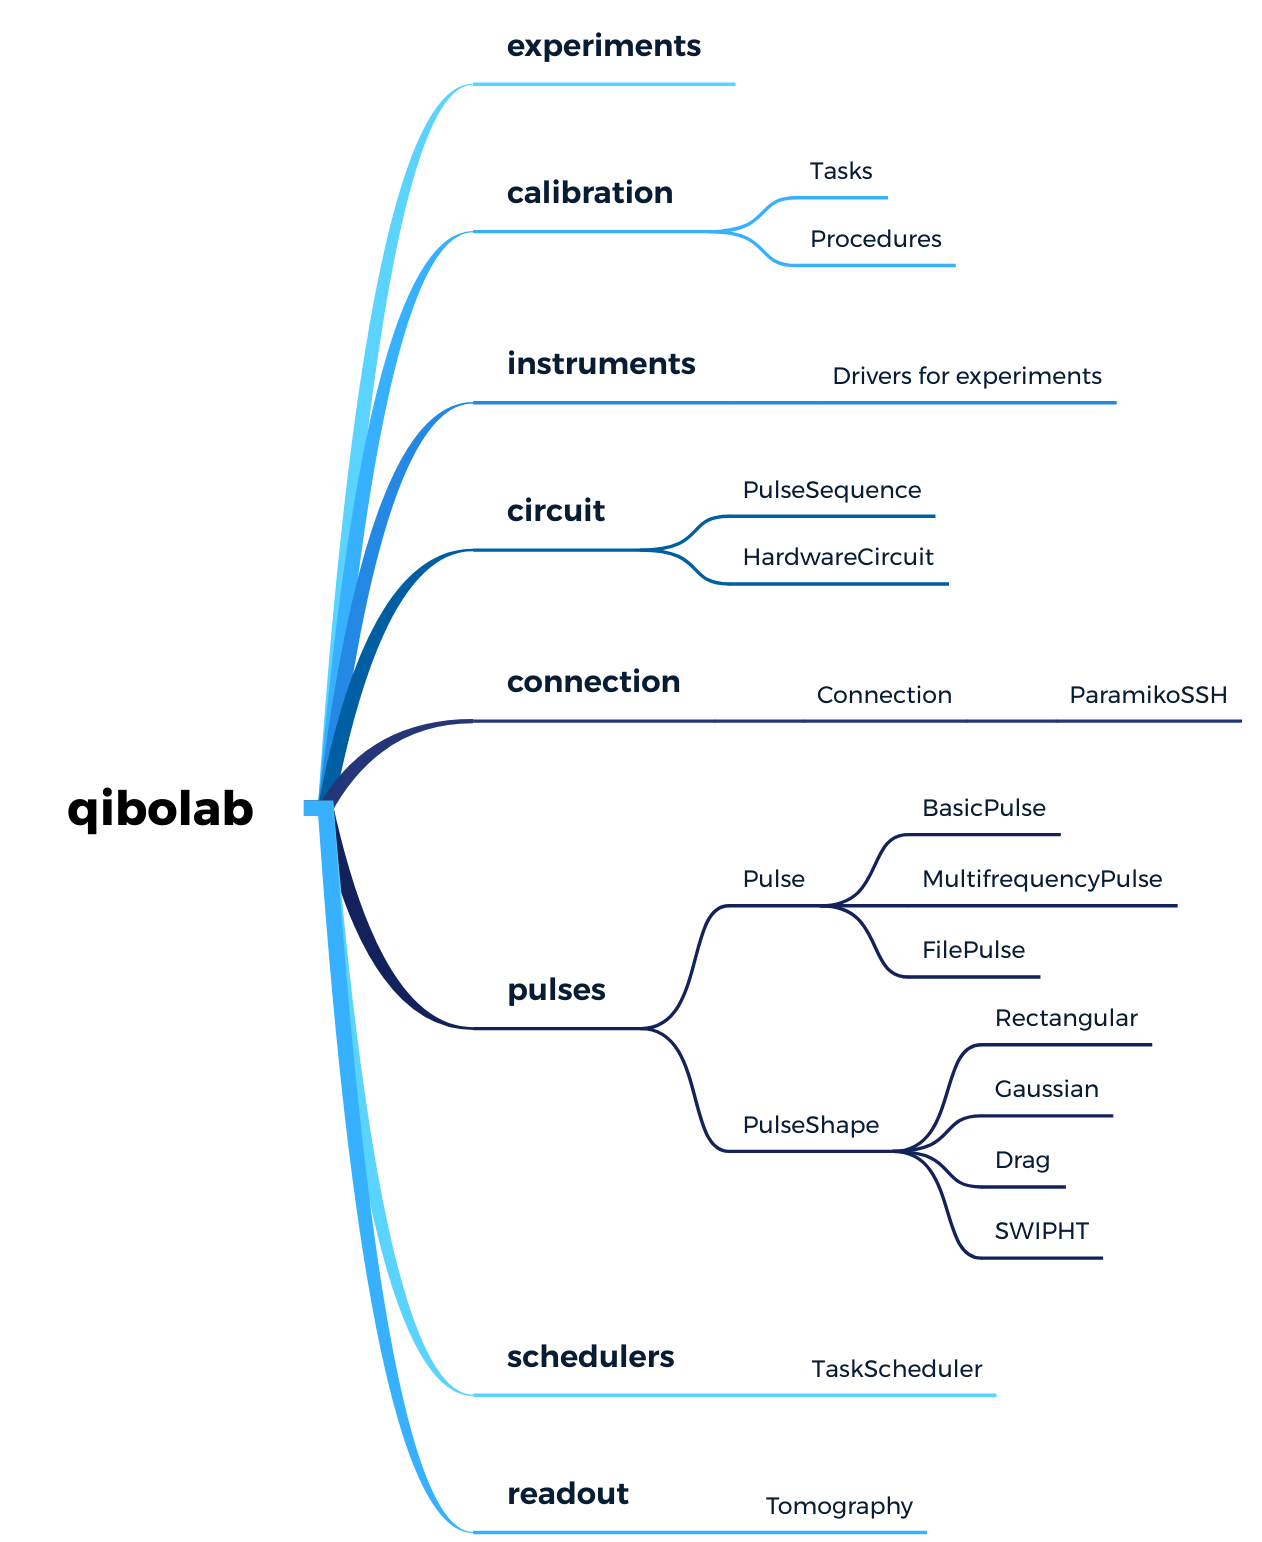
\includegraphics[height=0.8\textheight]{figures/qibolab.png}
            \end{figure}
            
        \end{column}

        \begin{column}[]{0.5 \textwidth}
            \begin{tcolorbox}[colframe=gray,title=Qibolab features:]
                \begin{itemize}
                    \item Deploy Qibo models on quantum hardware easily
                    \item User-friendly Pulse API
                    \item Create custom experimental drivers for lab setup
                    \item Support multiple heterogeneous platforms
                \end{itemize}
                \end{tcolorbox}
        \end{column}
    \end{columns}
\end{frame}

\begin{frame}{How to use qibolab?}
    \begin{figure}
        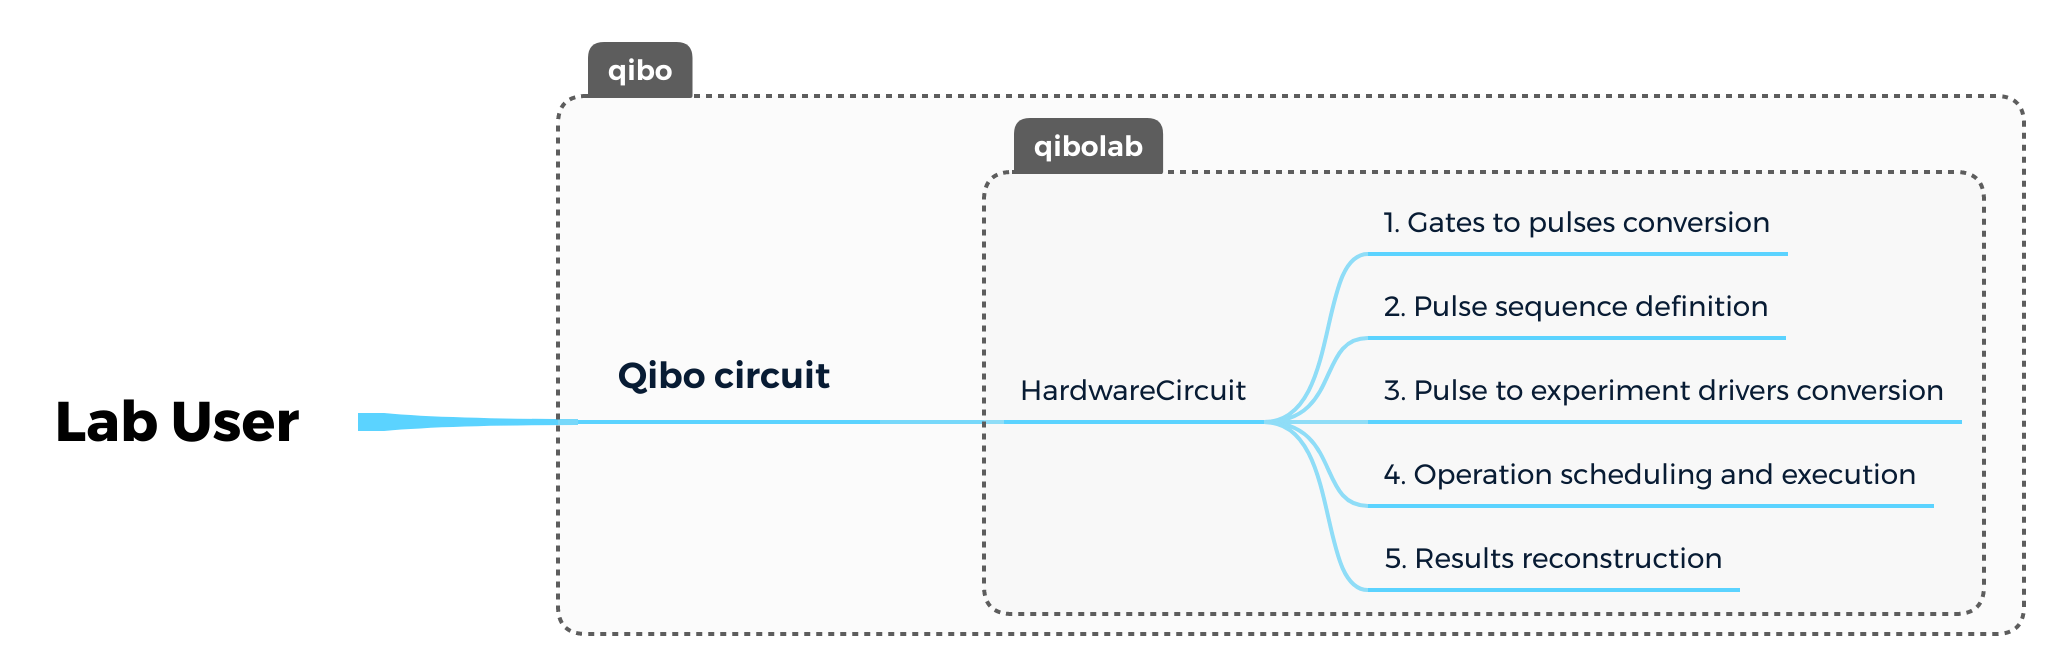
\includegraphics[width=\textwidth]{figures/hardwarecircuit.png}
    \end{figure}

    \begin{columns}
        \begin{column}{0.5 \textwidth}
            \begin{figure}
                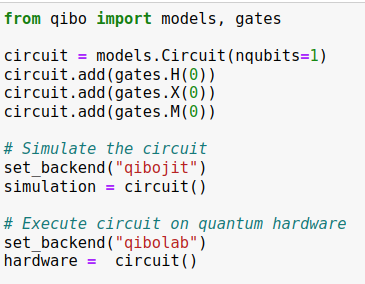
\includegraphics[width = \columnwidth]{figures/qibo__circuit.png}
            \end{figure}
        \end{column}
        \begin{column}{0.5 \textwidth}
            \begin{itemize}
                \item A single object to execute both on hardware and simulation
                \item Job scheduling to access the hardware using slurm
            \end{itemize}
            \centering
            
\includegraphics[height=2cm]{figures/Slurm_logo.svg.png}
        \end{column}
    \end{columns}

\end{frame}

\begin{frame}{Quantum Machine Learning on Real Hardware}
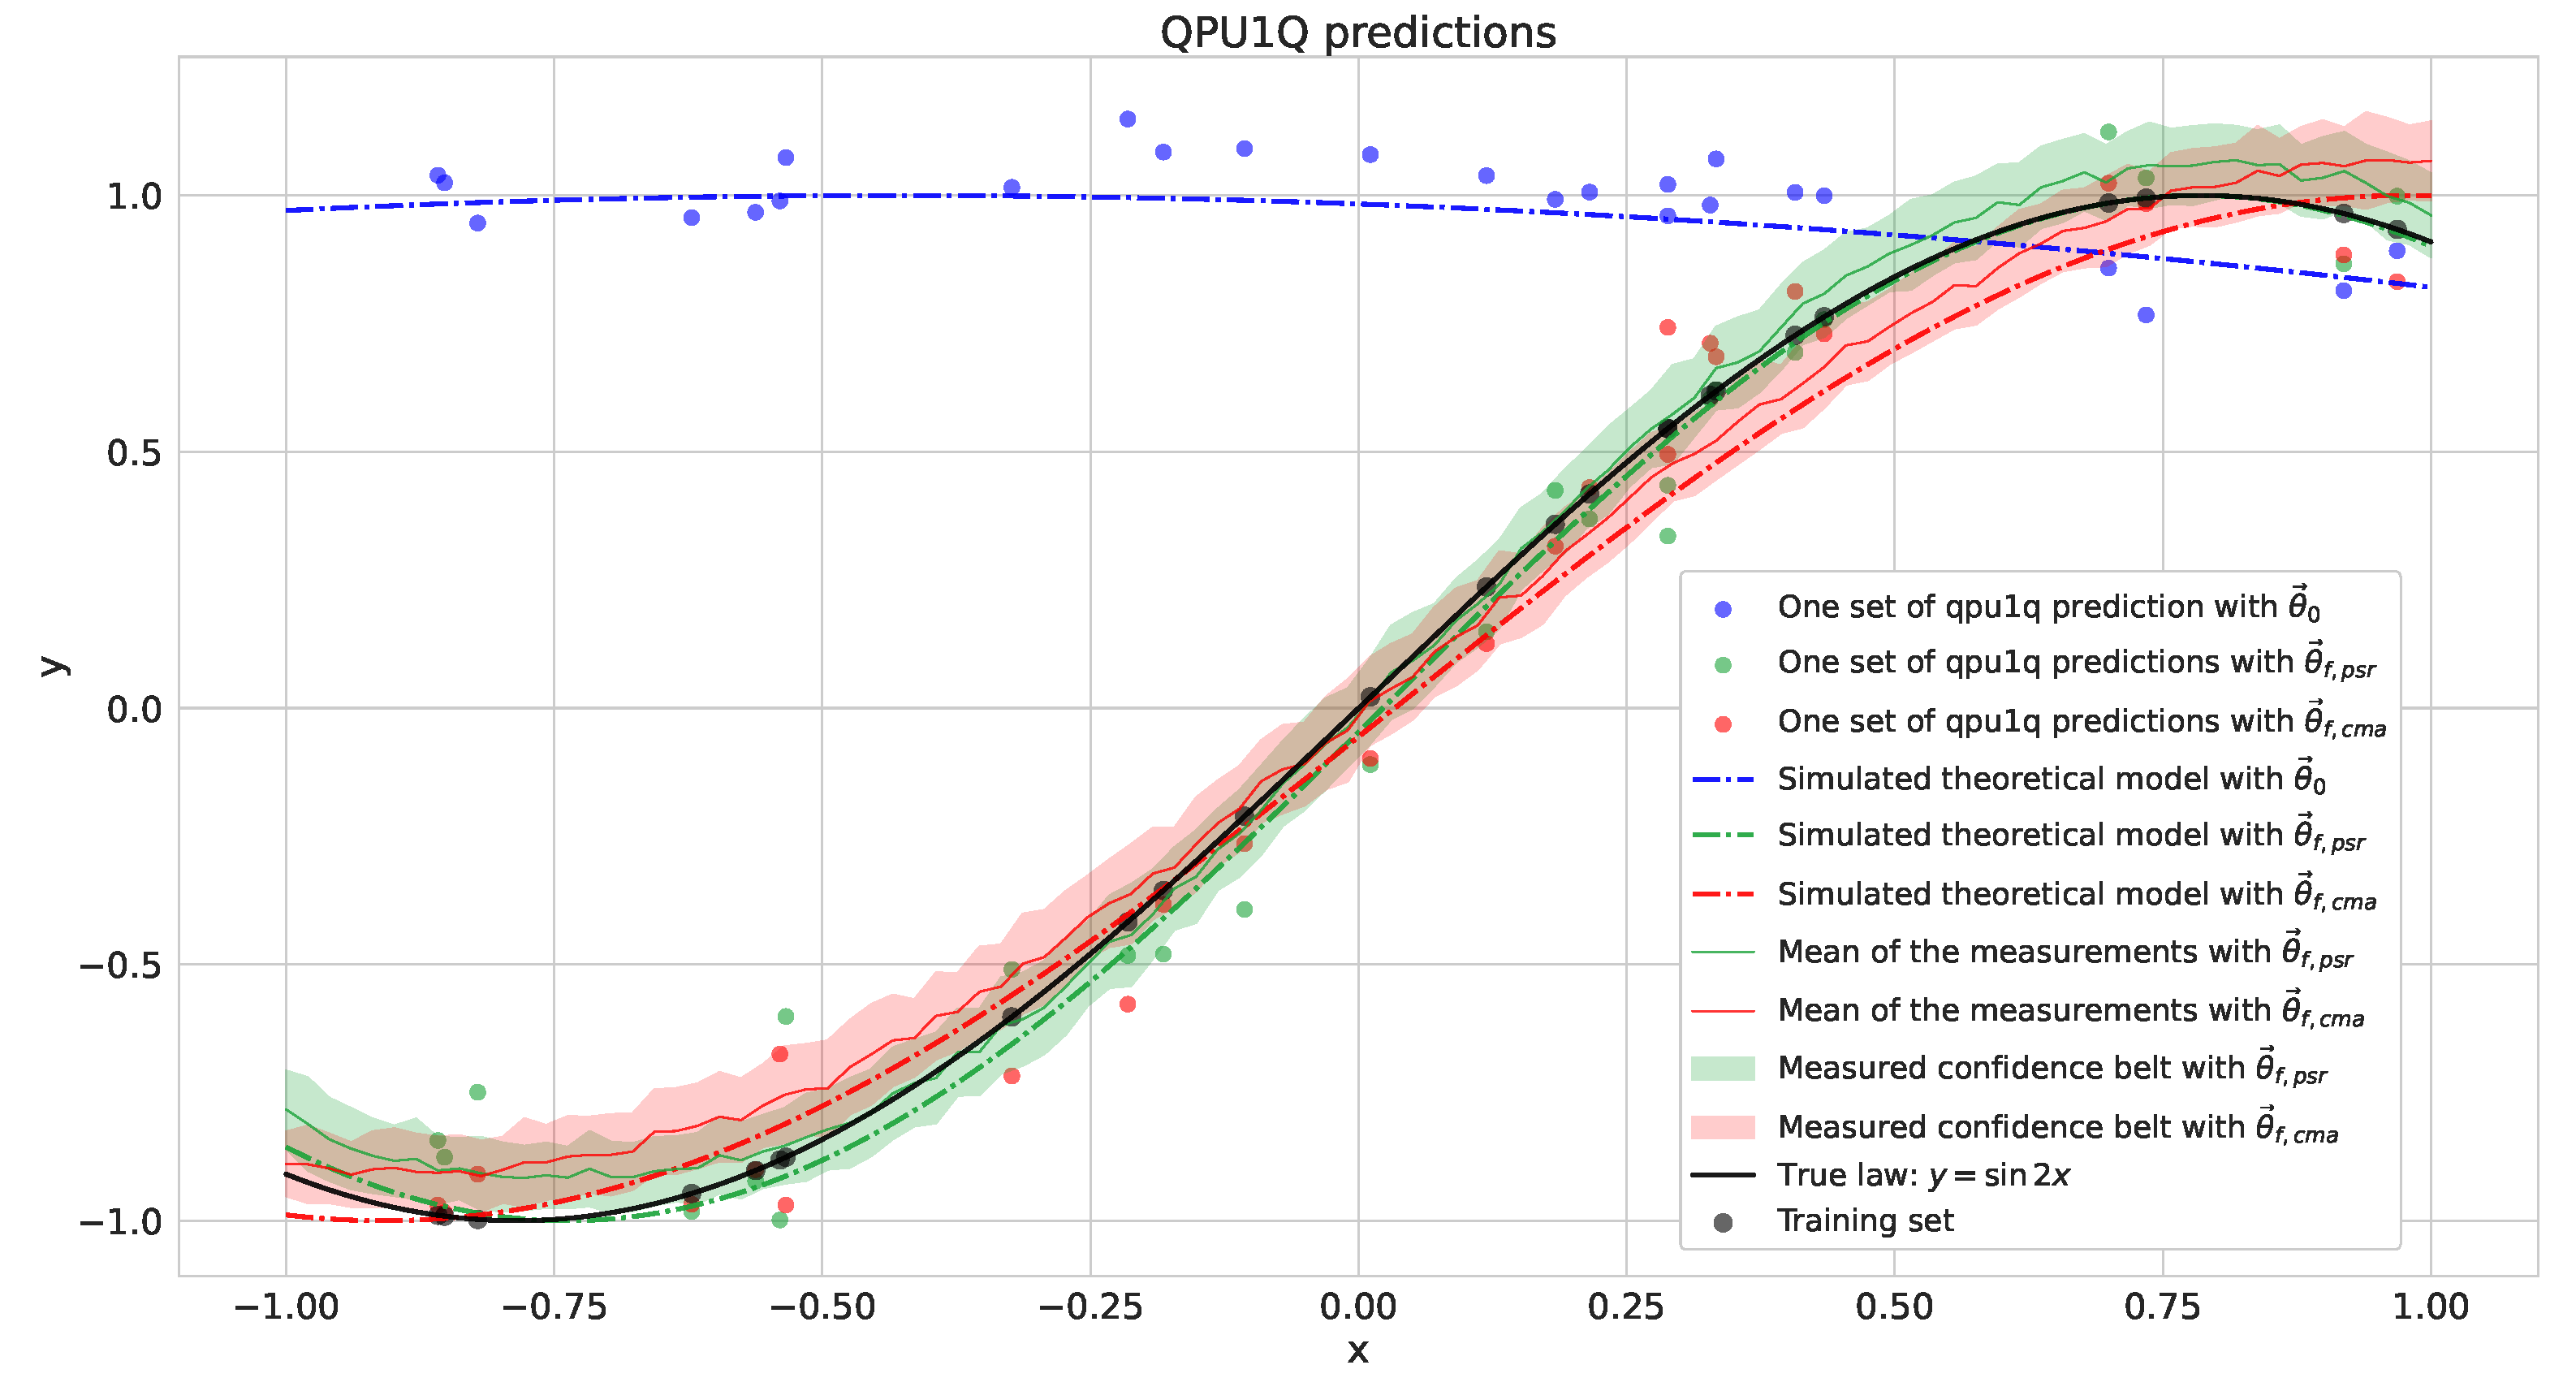
\includegraphics[width=\textwidth]{figures/cropped_qpu_not_normed..pdf}
\end{frame}



\section{A reporting tool for calibration using Qibo}

\begin{frame}{Difficulties}
    Suppose that we have assembled a quantum computer and we have a way
    to send pulses to the chip... are we done? {\color{red} \textbf{No} }

    We need to { \color{blue} characterize}, { \color{blue} validate} and { \color{blue} verificate} our qubits (QCVV):
    \begin{columns}
        \begin{column}{0.5 \textwidth}
            \vspace{-2cm}
            \begin{itemize}
                \item[\faCaretSquareORight] Perform standard calibration routines:
                \begin{itemize}
                    \item[\faWrench] Resonator and qubit spectroscopy
                    \item[\faWrench] Rabi and Ramsey 
                    \item[\faWrench] T1 and T2 determination
                
                \end{itemize}
                \item[\faCaretSquareORight] Perform quantum protocols to extract the fidelity:
                \begin{itemize}
                    \item[\faWrench] Randomized Benchmarking
                    \item[\faWrench] Gate Set Tomography
                    \item[\faWrench] Cross-Entropy Benchmarking
                \end{itemize}
                \item[\faCaretSquareORight] Repeat the above steps periodically.
            \end{itemize}
        \end{column}
        \begin{column}{0.5 \textwidth}
            \begin{figure}
                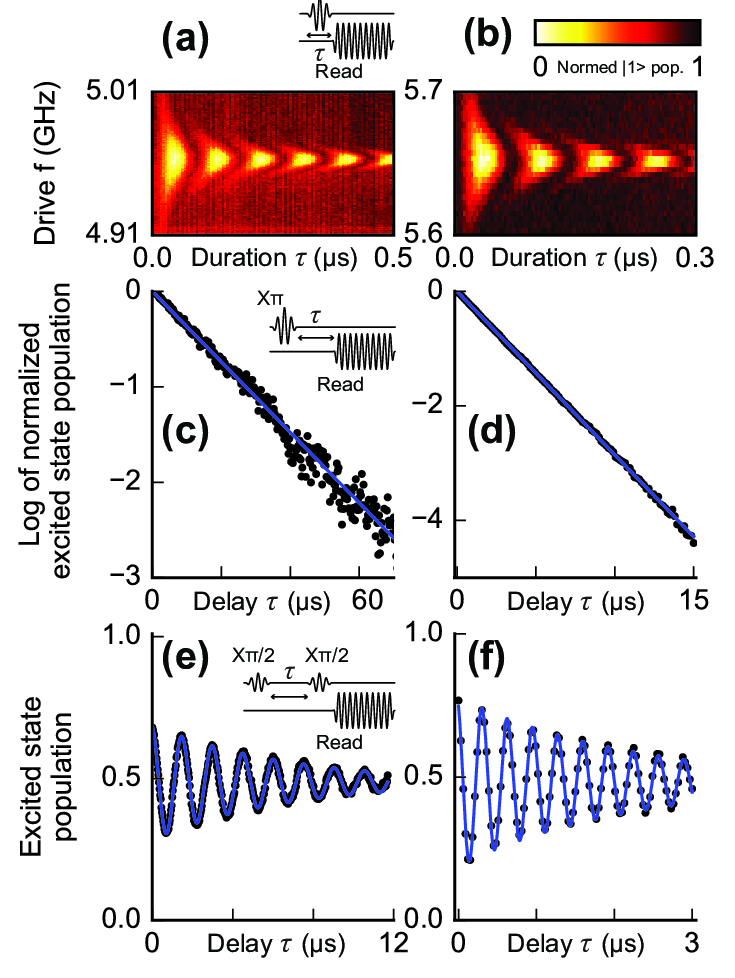
\includegraphics[width = 0.8 \textwidth]{figures/characterization.png}
            \end{figure}
            
        \end{column}
    \end{columns}
    

\end{frame}

\begin{frame}{A new reporting tool for Qibo}
    We are developing a new tool that it will be able to perform QCVV in Qibo
    with the following features:
            \begin{multicols*}{2}
                \begin{itemize}
                    \item[\faCaretSquareORight] Platform agnostic
                    \item[\faCaretSquareORight] Launch calibration routine easily
                    \item[\faCaretSquareORight] Live-plotting tools
                    \item[\faCaretSquareORight] Live-fitting tools
                    \item[\faCaretSquareORight]Save and share your data
                    \item[\faCaretSquareORight] Autocalibration routines
                \end{itemize}
            \end{multicols*}
            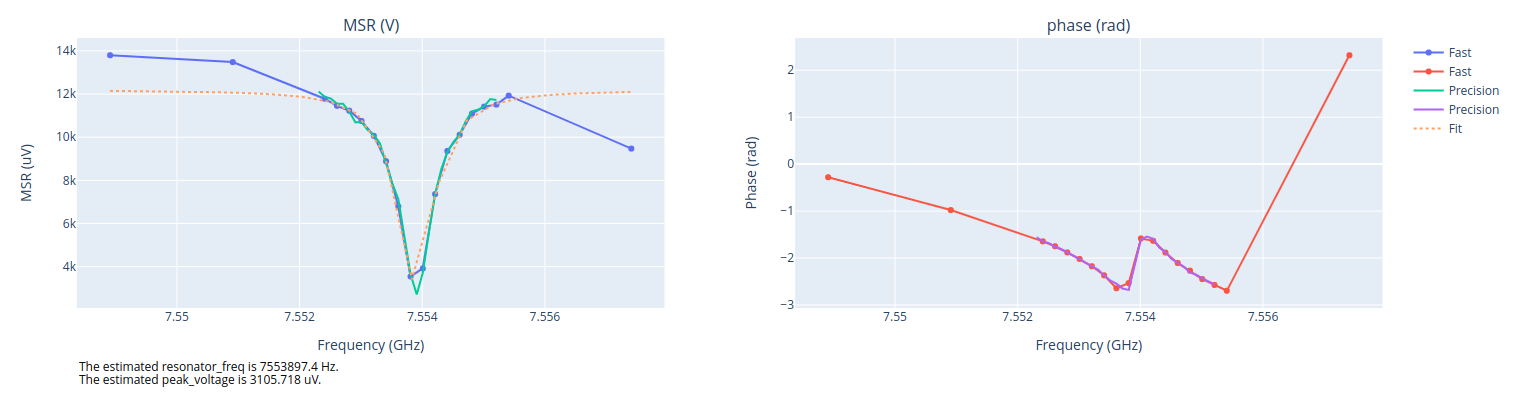
\includegraphics[width=\textwidth]{figures/resonator.png}
            

   
\end{frame}

\begin{frame}{Report example}
    
    \begin{figure}
        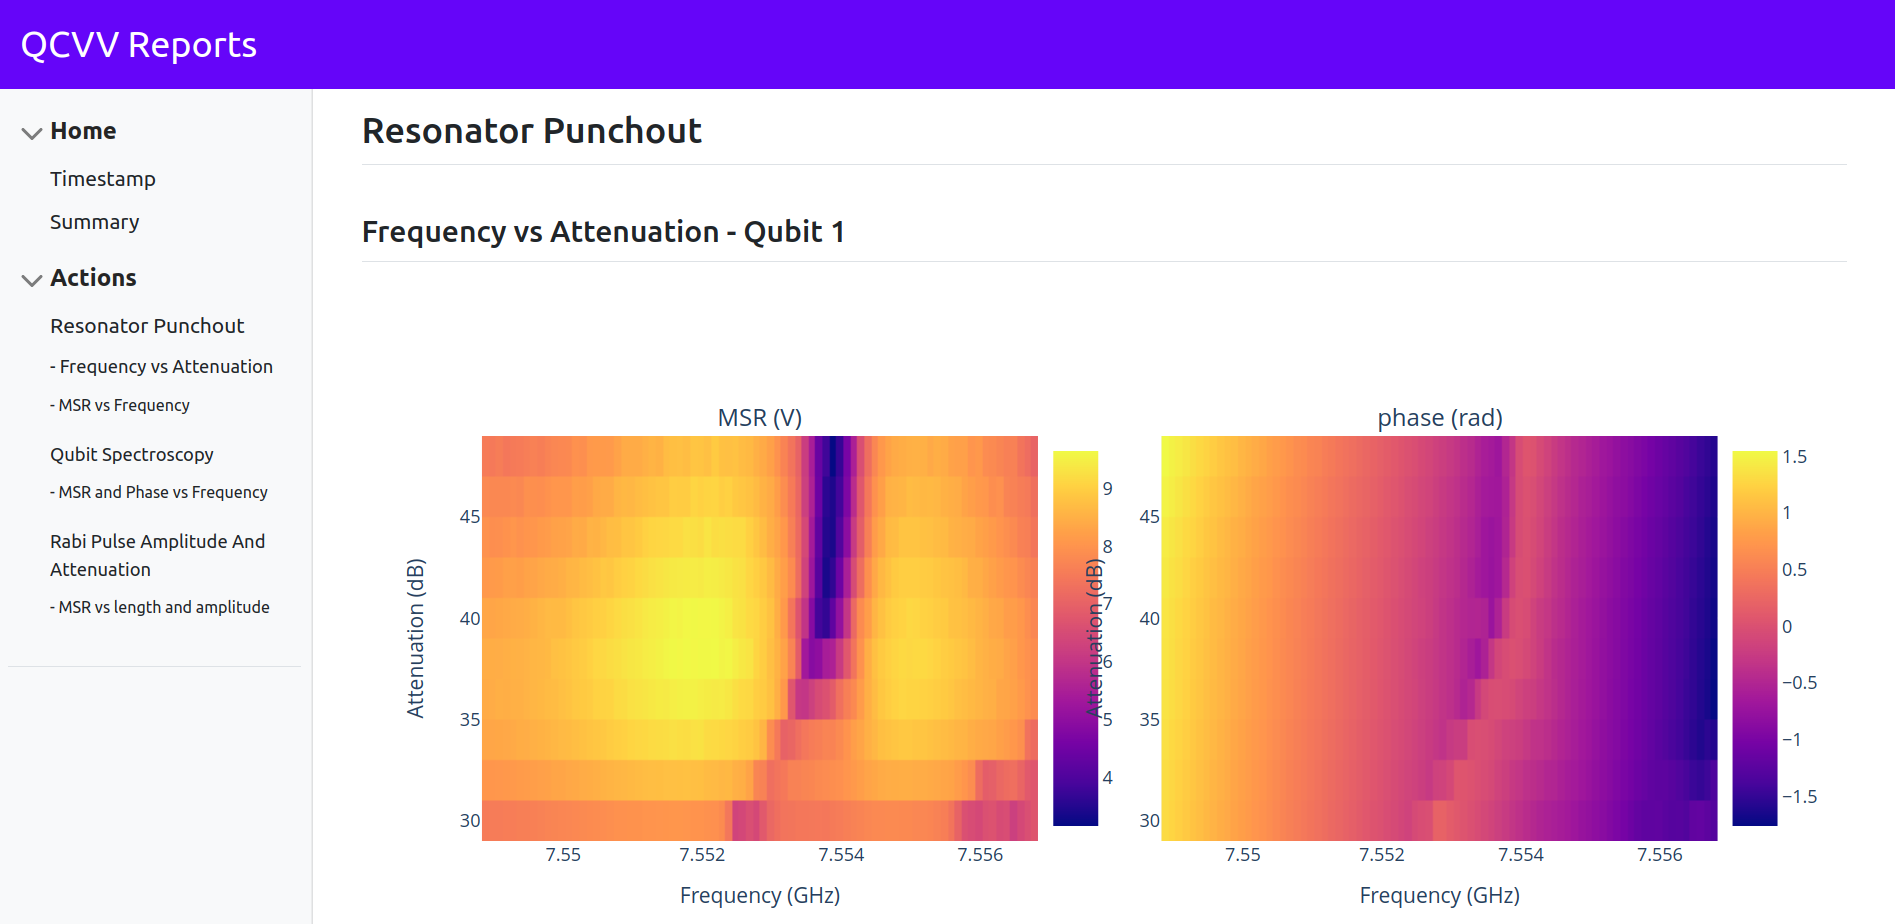
\includegraphics[width=\textwidth]{figures/qcvv.png}
        % 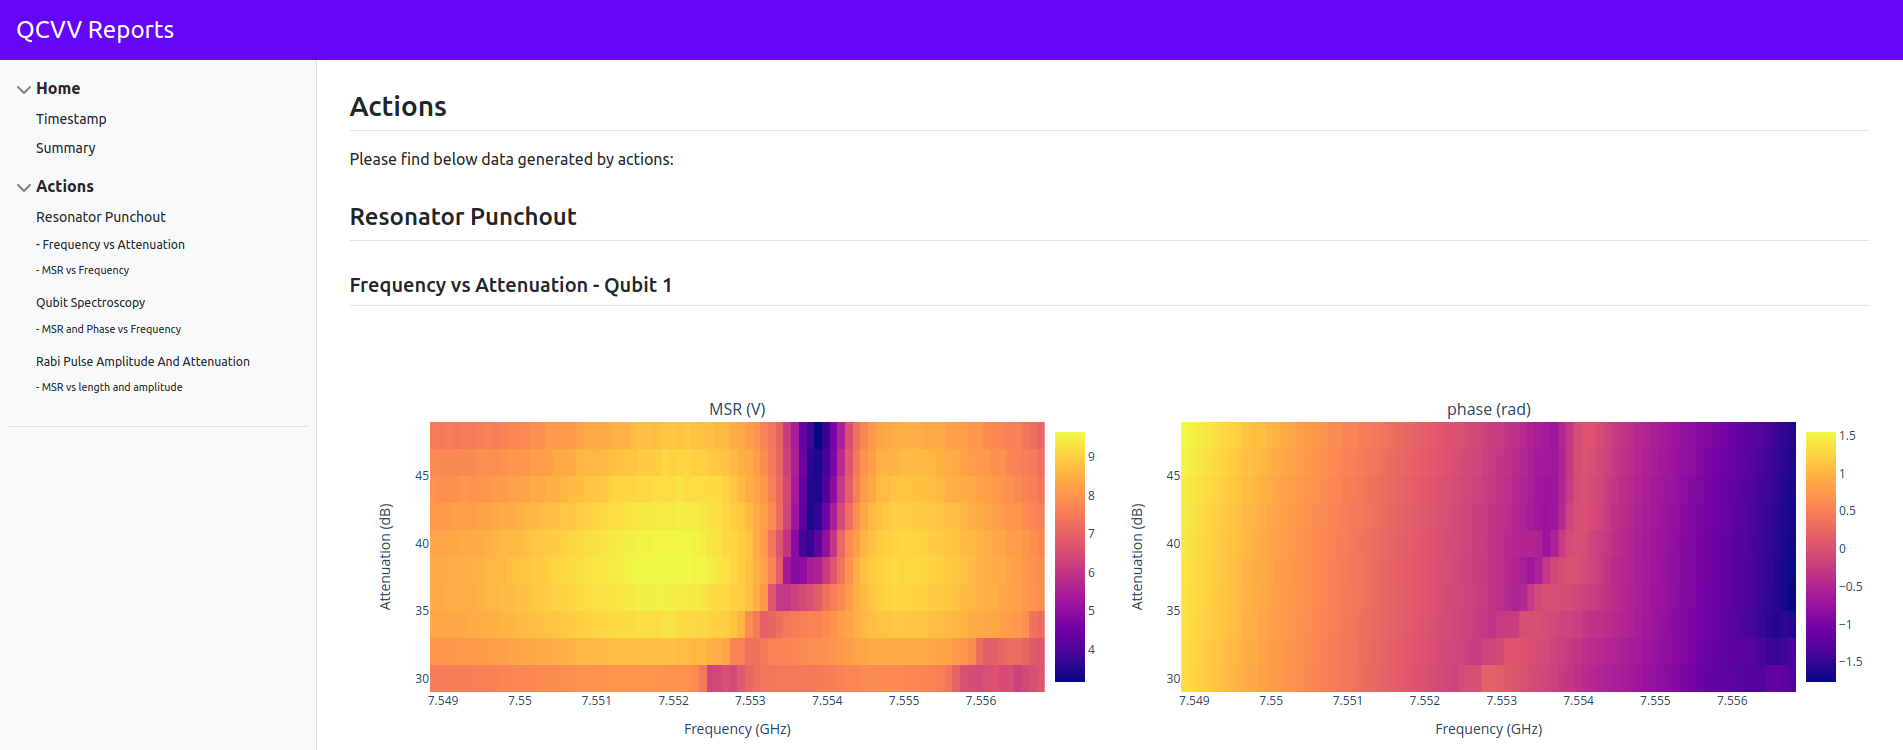
\includegraphics[width=\textwidth]{figures/punchout.png}
    \end{figure}
    
\end{frame}
\section{Outlook}

\begin{frame}{Outlook}
    Qibo is growing to accomodate different tasks:
    \begin{wrapfigure}{r}{0.25\textwidth}
        
\includegraphics[width=0.9\linewidth]{figures/qibo_logo.png} 
        \end{wrapfigure}
    \begin{itemize}
        \item[ \color{teal} \faCheck] High-performance quantum simulation: {\color{blue} \textbf{qibojit}}
        \item[ \color{orange}\faCheck] Hardware control: {\color{red} \textbf{qibolab}}
        \item[ \color{orange} \faCheck] Hardware calibration: { \color{teal} \textbf{qcvv} }
    \end{itemize}

    What makes Qibo different from other libraries:
    \begin{itemize}
        \item[ \faPlus] Public available as an open source project.
        \item[ \faPlus] Modular layout design with possibility of adding
        \begin{itemize}
            \item a new backend for simulation
            \item a new platform for hardware control
        \end{itemize}
        \item[ \faPlus] Community driven effort
    \end{itemize}

    \url{https://github.com/qiboteam/qibo} \hfill \url{https://qibo.readthedocs.io/en/stable/}
\end{frame}
\section{Thanks for listening!}
\end{document}